% Formatted using uploaded MATH_4890_dissertation_template.zip, 15 November 2026.
% Analytical supplement, 15 November 2026. Frozen scope and all inherited records retained.
% Dissertation source, 2 November 2026.
% Goal: reduce complex PDEs to simpler forms and obtain exact or approximate analytical solutions.
% Inherited numerical evidence and frozen research records stay unchanged. New proved supplements use independent counters.
% Compile: latexmk -pdf -interaction=nonstopmode -halt-on-error dissertation_wku.tex
% Revision: motivations aligned with parameters, symmetry structure and series geometry.
% Existing numbered equations, theorem environments and embedded plot data retained.
% Figure edits follow docs/dissertation-figure-workflow.md.
\documentclass[12pt,a4paper,oneside]{report}
\usepackage[T1]{fontenc}
\usepackage[utf8]{inputenc}
\usepackage{lmodern}
\usepackage[nopatch=footnote]{microtype}
\usepackage[top=1in,bottom=0.689in,hmargin=1.25in,nohead,includefoot,foot=0.311in,footskip=0.5827in]{geometry}
\usepackage{amsmath,amssymb,amsthm,mathtools,mathrsfs}
\usepackage{booktabs,array,tabularx,longtable}
\renewcommand{\tabularxcolumn}[1]{>{\raggedright\arraybackslash}p{#1}}
\usepackage{graphicx,tikz,pgfplots,pgfplotstable,adjustbox}
\BeforeBeginEnvironment{tikzpicture}{\begin{adjustbox}{max width=\linewidth}}
\AfterEndEnvironment{tikzpicture}{\end{adjustbox}}
\usetikzlibrary{arrows.meta,positioning,calc}
\usepgfplotslibrary{groupplots}
\pgfplotsset{compat=1.18}
\usepackage[numbers,sort&compress]{natbib}
\usepackage[hyphens]{url}
\usepackage{hyperref,bookmark}
\usepackage{setspace,fancyhdr,titlesec,caption,placeins}
\definecolor{ink}{HTML}{263B5E}
\definecolor{teal}{HTML}{087F8C}
\definecolor{warm}{HTML}{B65528}
\hypersetup{colorlinks=true,linkcolor=ink,citecolor=teal,urlcolor=teal,
 pdfauthor={Yihong Xiao},
 pdftitle={Parameter-Dependent Lie Symmetries and Semi-Analytical Solutions of Nonlinear PDEs},
 pdfsubject={Undergraduate dissertation, MATH 4890}}
\titleformat{\chapter}[hang]{\normalfont\Large\bfseries\raggedright}{\thechapter.}{.7em}{}
\titlespacing*{\chapter}{0pt}{-20pt}{12pt}
\titleformat{\section}{\normalfont\large\bfseries}{\thesection}{.6em}{}
\titlespacing*{\section}{0pt}{8pt plus 2pt}{3pt}
\titlespacing*{\subsection}{0pt}{8pt plus 2pt}{3pt}
\captionsetup{font=small,labelfont=bf,skip=4pt}
\setlength{\textfloatsep}{10pt plus 2pt minus 2pt}
\setlength{\intextsep}{9pt plus 2pt minus 2pt}
\renewcommand{\topfraction}{.9}
\renewcommand{\textfraction}{.08}
\setstretch{1.0}
\setlength{\emergencystretch}{2em}
\setlength{\parskip}{0pt}
\setcounter{tocdepth}{2}
\makeatletter
\renewcommand{\@pnumwidth}{2.8em}
\renewcommand{\@tocrmarg}{3.8em}
\makeatother
\raggedbottom
\numberwithin{equation}{chapter}
\newtheorem{theorem}{Theorem}[chapter]
\newtheorem{proposition}[theorem]{Proposition}
\newtheorem{corollary}[theorem]{Corollary}
\newtheorem{definition}[theorem]{Definition}
\theoremstyle{remark}\newtheorem{remark}[theorem]{Remark}
\newcommand{\dd}{\,\mathrm d}
\newcommand{\E}{\mathcal E}
\newcommand{\pr}{\operatorname{pr}}
\newcommand{\rank}{\operatorname{rank}}
\newcommand{\norm}[1]{\left\lVert#1\right\rVert}
\DeclareRobustCommand{\code}[1]{\nolinkurl{#1}}
\newcommand{\doi}[1]{\href{https://doi.org/#1}{doi: #1}}
\pagestyle{fancy}\fancyhf{}
\renewcommand{\headrulewidth}{0pt}
\fancyfoot[R]{\thepage}
\fancypagestyle{plain}{\fancyhf{}\fancyfoot[R]{\thepage}\renewcommand{\headrulewidth}{0pt}}
\setlength{\tabcolsep}{1mm}
\renewcommand{\arraystretch}{1.3}
\renewcommand{\bibname}{References}
\renewcommand{\chaptermark}[1]{\markboth{\thechapter.\ #1}{}}
\tikzset{box/.style={draw=ink,fill=ink!4,rounded corners=2pt,
 align=center,inner sep=5pt,font=\small},
 planned/.style={box,draw=teal,fill=teal!5,dashed},
 arr/.style={-{Latex[length=2mm]},thick,ink},
 warnbox/.style={draw=warm,fill=warm!5,rounded corners=2pt,align=center,inner sep=4pt,font=\scriptsize},
 mlbox/.style={draw=teal,fill=teal!6,rounded corners=2pt,align=center,inner sep=4pt,font=\scriptsize},
 note/.style={font=\scriptsize,align=center},
 warr/.style={-{Latex[length=1.8mm]},thick,warm,dashed},
 tarr/.style={-{Latex[length=1.8mm]},thick,teal}}

\pgfplotstableread{
x profile profile_minus profile_plus residual residual_minus residual_plus seconds seconds_minus seconds_plus
1 1.1578960013025608e-11 1.0364820113295536e-11 2.9303448556561307e-11 8.9995959477274363e-08 4.6121937078016027e-09 1.514146122817689e-07 0.10403072700023586 0.026213287000018681 0.15741335699999581
2 1.830091633792108e-12 1.2074785615823203e-12 8.9310780992946093e-12 7.88473941975085e-09 3.5439069124312552e-09 9.3784724610635164e-10 0.22343795500000851 0.012908440000046539 0.017612406000353076
3 2.4424906541753444e-15 6.6613381477509392e-16 6.6613381477509392e-16 1.2674076345104898e-11 7.1467057719102429e-13 7.1467057719102429e-13 0.28584620549986539 0.009994795500233522 0.009994795500233522
4 2.1195447806876544e-05 1.8442921475125829e-05 9.8612344845427913e-07 0.0010640066634975895 0.00021124565787272818 0.0043612627281888793 0.037473304499826554 0.0053431485000601242 0.0086267545000282553
}\ComparisonP

\pgfplotstableread{
x profile profile_minus profile_plus residual residual_minus residual_plus seconds seconds_minus seconds_plus
1 1.2187406639441178e-10 7.4306338859742027e-11 2.3218005296143929e-10 3.0668566415080427e-06 2.8641460855777032e-07 3.8152263379575551e-06 0.19486531450002076 0.041828088500096783 0.086359378500219464
2 7.2046146826210133e-11 5.7884141924091637e-11 1.8703483206650162e-11 4.5323017128231256e-07 2.4057306490752602e-07 6.3223880825705451e-08 0.25119437900002595 0.0085935609999978624 0.04913098999986687
3 1.6120438317557273e-13 6.2172489379008766e-15 6.2172489379008766e-15 3.1065171370379012e-09 1.0954283410336634e-10 1.0954283410336634e-10 0.29183370949999698 0.0078219194999746833 0.0078219194999746833
4 3.6590460728902485e-05 1.8683035256650271e-06 8.0498807178752685e-05 0.021317858560875633 0.00705454365320002 0.012384013940556125 0.041675711500147372 0.0039696195001397427 0.0056258494998928654
}\ComparisonM

% Independent counters keep all inherited theorem numbers unchanged.
\newtheorem{suppprop}{Proposition}[chapter]
\renewcommand{\thesuppprop}{\thechapter.\Alph{suppprop}}
\newtheorem{supptheorem}[suppprop]{Theorem}

\begin{document}
\hypersetup{pageanchor=false}
\pagenumbering{Roman}
\begin{titlepage}
\thispagestyle{plain}
\noindent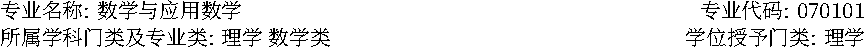
\includegraphics[width=\textwidth]{wku_programme_header.pdf}
\vspace{18mm}
\begin{center}
\textbf{College of Science, Mathematics and Technology}\par
\medskip
\textbf{Wenzhou-Kean University}\par
\vspace{8mm}

\includegraphics[width=2.2055in,height=1.9055in]{WKU.png}\par
\vspace{25mm}
{\bfseries Parameter-Dependent Lie Symmetries\par
and Semi-Analytical Solutions\par
of Nonlinear PDEs\par}
\vspace{4mm}
Saint--Venant--Exner Case Studies\par
{\small Lie-Invariant Reference Families and Targeted Corrections\par}
\vspace{3mm}
Undergraduate Dissertation (MATH 4890)
\end{center}
\vspace{10mm}
\noindent\begin{tabularx}{\textwidth}{@{}lX@{}}
\textbf{Student Name:} & \underline{Yihong Xiao}\\[4pt]
\textbf{Student ID:} & \underline{1308225}\\[4pt]
\textbf{Major:} & \underline{Mathematical Sciences}\\[-2pt]
 & \underline{(Data Analytics Option)}\\[4pt]
\textbf{Supervisor:} & \underline{Dr.\ Puneet Rana}\\[4pt]
\textbf{Date of Submission:} & \underline{11 November 2026}
\end{tabularx}
\end{titlepage}
\hypersetup{pageanchor=true}
\setcounter{page}{2}
\chapter*{Author's Declaration}
\addcontentsline{toc}{chapter}{Author's Declaration}
I, the undersigned, hereby declare that this submission is entirely my own work, in my own words, and that all sources used in researching it are fully acknowledged and all quotations properly identified. It has not been submitted, in whole or in part, by me or another person, for the purpose of obtaining any other credit/grade. I have a citation to AI system used to generate the text if I used AI-generated text. I understand the ethical implications of my research, and this work meets the requirements of College of Science, Mathematics and Technology.

\vspace{25mm}
\noindent\textbf{Date:} \rule[-8pt]{11.5cm}{0.1em}\par
\bigskip\bigskip
\noindent\textbf{Name (printed letters):} \rule[-8pt]{7.8cm}{0.1em}\par
\bigskip\bigskip
\noindent\textbf{Signature:} \rule[-8pt]{10.55cm}{0.1em}
\vfill
{\small\noindent\textit{AI assistance disclosure.} OpenAI ChatGPT was used for drafting,
mathematical exposition, verification-code preparation and typesetting assistance
in this document (November 2026; \url{https://chatgpt.com/}). The declaration
above remains unsigned for the author's review.}
\clearpage
\chapter*{Abstract}
\addcontentsline{toc}{chapter}{Abstract}
This dissertation develops a structure-aware approach to semi-analytical solution construction for nonlinear partial differential equations. The organizing question is whether verified Lie-invariant reference families can support controlled approximation and targeted corrections beyond a selected invariant class. The one-dimensional Grass-type Saint--Venant--Exner system is the main model. Conservation laws, constitutive assumptions and a locally invertible mass coordinate determine a compatible material scalar equation. A different printed scalar benchmark is retained only for source comparison and historical experiments.

The method first verifies a symmetry and the conditions for invariant-graph reduction, solves the resulting ordinary differential equation by integration or local series, and reconstructs the physical fields. A material travelling-wave family supplies an explicit regular example. The cubic scaling supplies a two-parameter convergent Laurent branch on a restricted parameter stratum; it does not exhaust the third-order reduced equation. Derivative bounds and coordinate inversion are required to translate profile accuracy into physical accuracy.

A second stage formulates corrections for changed parameters or non-invariant data. Local coordinates separate reference-family parameters from a complementary function-space direction. A conditional contraction proposition states sufficient conditions for validation, but its infinite-dimensional hypotheses have not yet been established for the implemented SVE problem. Machine learning supplies candidate corrections and is compared with a direct neural baseline and a shared classical corrector. The current implementation covers a regular exponent-one reference family; neither a measured learning advantage nor continuous PDE certification is claimed.

The original two-dimensional annular continuation analysis and scalar approximation records are retained as explicitly separate extensions. The resulting contribution is a model-specific analytical foundation and a testable correction architecture, not a general nonlinear PDE solver.

\medskip\noindent\textbf{Keywords:} Lie symmetry; invariant reduction; Saint--Venant--Exner system; Laurent series; physical reconstruction; learning-assisted correction.
\clearpage
\tableofcontents
\clearpage
\addcontentsline{toc}{chapter}{List of Figures}
\listoffigures
\clearpage
\addcontentsline{toc}{chapter}{List of Tables}
\listoftables
\clearpage
\chapter*{List of Symbols and Abbreviations}\label{sec:notation}
\addcontentsline{toc}{chapter}{List of Symbols and Abbreviations}
\begin{table}[h!]\centering\small
\begin{tabularx}{\textwidth}{@{}p{.25\textwidth}X@{}}\toprule
Symbol & Meaning (the context specifies its domain)\\\midrule
$E_1(=E),E_2$ & One-dimensional and two-dimensional SVE systems, both in Eulerian descriptions. $E_2$ is written in Cartesian coordinates and later reduced in polar coordinates.\\
$M,P$ & Compatible one-dimensional Lagrangian/material scalar equation and distinct printed scalar benchmark; these are \emph{model names}.\\
$\Delta[U]$, $\mathscr E_\Delta$ & Differential PDE residual evaluated at $U$, and its zero \emph{equation locus} in a jet bundle. Square brackets mean evaluation, not commutation.\\
$\mathcal E_m^{\mathrm c}[\phi]$, $\mathcal E_m^{\mathrm p}[\phi]$ & Material scalar residuals of $M$ and $P$, respectively.\\
$\mathcal R_m[F]$ & Reduced similarity-ODE residual (not a rotation vector field).\\
$X$, $\operatorname{pr}^{(n)}X$, $Q_X$ & Symmetry generator, its prolongation and invariant-surface characteristic.\\
$\mathfrak g$, $\mathfrak h$; $p,k$ & Admitted Lie algebra, selected subalgebra; numbers of base variables and transverse group-orbit dimensions.\\
$(t,s,\phi)$; $z,F$ & One-dimensional material coordinates and particle map; similarity invariant and profile.\\
$(t,x,y)$; $h,\mathbf w,B$ & Two-dimensional \emph{Eulerian--Cartesian} space--time, depth, horizontal velocity and bed elevation.\\
$r,H,V,W,Z$ & Annular radius, water-depth profile, radial and azimuthal velocities, bed profile.\\
$Q$, $S$, $P_Z$ & Annular sediment flux, squared speed $S=V^2+W^2$, and bed slope $Z'=P_Z(r,H)$. These symbols are not model $P$. The one-dimensional letters $T,S,U,D$ and the relative speed $V=F-zp$ are local to their own sections.\\
$D,N$ & $D=gH-V^2$ and right-hand side of the undivided radial equation $DH'=N$.\\
$\lambda$, $\theta$, $\widehat H_\theta$ & Physical/IVP parameter vector, fitted coefficients, and candidate reduced profile.\\\bottomrule
\end{tabularx}
\caption[Symbols and notation]{Symbols used repeatedly; remaining local symbols are defined with their equations.}
\end{table}
\noindent\emph{Example:} $\Delta[U]=0$ asserts the original system,
$Q_X[U]=0$ selects one of its invariant solution classes, and
$\mathcal R_m[F]=0$ is a resulting one-dimensional profile equation.


\clearpage
\pagenumbering{arabic}
% Begin sections/01-introduction.tex
\chapter{Introduction}\label{ch:introduction}
\section{Research setting and computational motivation}
Nonlinear PDEs in mathematical physics and engineering often contain
constitutive parameters whose variation changes the available analytical
structure. The aim here is to reduce such equations and obtain exact or
controlled approximate analytical solutions. Specified frictionless,
depth-averaged Saint--Venant--Exner (SVE) systems provide concrete examples:
water transports sediment while the evolving bed feeds back into momentum
\cite{exner1925,fernandez2017}.

Physics-informed approximation motivates using analytical structure before
optimization. Composite training losses can suffer from unbalanced gradients
\cite{wang2020}; a small sampled loss alone does not certify a solution
\cite{mishra2023}. The proposed response is to eliminate symmetry directions
and integrate exact relations before approximating a remaining profile.
This complements classical integration and spectral approximation. Learning
is optional and must justify its additional cost against these controls.
No unverified industrial speedup or universal PINN failure rate is used as
evidence for the present method.

The intended application range is one to three spatial dimensions, with
time counted separately; this dissertation demonstrates only specified
one- and two-dimensional models. Low dimension alone does not guarantee
accuracy or efficiency: usable symmetries, compatible data, regularity and
conditioning remain necessary considerations. High dimension likewise does
not create an absolute impossibility of mesh-based computation. The
advantage investigated here is analytical structure within selected solution
classes, not a universal dimensional advantage over finite elements or PINNs.

\section{Three motivations and their mathematical scope}
For a parameterized system $\Delta_\lambda(x,j^nU)=0$, let
$\mathfrak g_\lambda$ denote its admitted point-symmetry algebra. The research
is organized by the following three motivations.
\begin{center}\small
\begin{tabularx}{\textwidth}{@{}p{.20\textwidth}XX@{}}\toprule
Motivation & Mathematical objective & Evidence in this dissertation\\\midrule
Parameters & Identify parameter strata and changes in regularity or admissible reductions & Restricted scalar strata; exponent regularity; an exact critical parameter family\\
Symmetry structure & Determine independent generators, brackets, subgroup equivalence and orbit rank & A restricted optimal system and a verified rank-two annular quotient\\
Series and geometry & Relate coefficient recurrences to singular loci, branches and continuation & Regular local series; a characteristic identity; two smooth critical germs\\\bottomrule
\end{tabularx}
\end{center}
These are related questions, not a proved universal implication from a
parameter change to a symmetry jump and then to a solution singularity.
A finite algebra dimension, an orbit rank and infinitely many series terms
measure different objects. A finite-order regular ODE may have an infinite
Taylor expansion determined by finitely many initial values.

For $p$ independent variables, a regular transverse subgroup of base-orbit
rank $k$ leaves $p-k$ variables. The annular example has $(p,k)=(3,2)$;
a one-dimensional optimal system alone does not classify its rank-two
reductions. The returned six-dimensional algebra belongs to a declared
shared affine class. Unrestricted maximality, exclusion of functional
symmetries and a complete optimal system remain open.

Reconstruction is the final consistency step: a reduced profile must yield
a solution of the stated original PDE. It is not a fourth motivation or
a substitute for the study of series geometry. Figure~\ref{fig:chain}
shows the computational workflow implementing the three motivations.

\begin{figure}[!htb]\centering
\begin{tikzpicture}[x=1cm,y=1cm,
  stage/.style={box,text width=10.4cm,minimum height=.7cm,font=\footnotesize},
  branch/.style={box,text width=4.65cm,minimum height=1.10cm,inner sep=4pt,font=\scriptsize},
  endstage/.style={box,text width=10.4cm,minimum height=.67cm,font=\footnotesize}]
 \node[stage] (m) at (0,0) {\textbf{1. Model and data:} $\Delta[U]=0$;\\ constitutive parameters, wet chart and invariant domain};
 \node[stage] (s) at (0,-1.18) {\textbf{2. Symmetry:} solve determining equations;\\ verify brackets and declared classification scope};
 \node[stage] (q) at (0,-2.36) {\textbf{3. Similarity quotient:} select $\mathfrak h$, impose $Q_X=0$ and rank/data gates};
 \node[stage] (o) at (0,-3.54) {\textbf{4. Exact order lowering:} $rHV=C_1$, $rW+fr^2/2=C_2$, $rQ+cr^2/2=C_3$};
 \node[branch,draw=teal,fill=teal!7] (a) at (-5.15,-5.23) {\textbf{A. Analytical track}\\undivided $DH'=N$; first integrals;\\ Taylor coefficients; saddle theorem};
 \node[branch,draw=teal,fill=teal!5,dashed] (l) at (0,-5.23) {\textbf{B. Optional learned track}\\$\widehat H_\theta=P_k+\rho^{k+1}N_\theta$;\\ fit coefficients on a regular chart};
 \node[branch,draw=ink,fill=ink!3] (c) at (5.15,-5.23) {\textbf{C. Classical control}\\DOP853, Taylor, \mbox{Chebyshev}; same initial data and numerical tolerances};
 \node[endstage] (r) at (0,-7.06) {\textbf{5. Reconstruct:} $\widehat V,\widehat W,\widehat Z$ from exact currents and verified quadrature};
 \node[endstage] (v) at (0,-8.25) {\textbf{6. Independent validation:} continuous residual, parameter tube;\\ all Cartesian PDE equations};
 \node[endstage] (z) at (0,-9.43) {\textbf{7. Report:} proved / verified / fitted / failed;\\ total costs, guards and domain};
 \draw[arr] (m)--(s);\draw[arr] (s)--(q);\draw[arr] (q)--(o);
 \draw[arr] (o.south) -- (0,-4.23) -| (a.north);
 \draw[tarr] (o.south) -- (l.north);
 \draw[arr] (o.south) -- (0,-4.23) -| (c.north);
 \draw[ink,thick] (-5.15,-6.23)--(5.15,-6.23);
 \draw[arr] (a.south)--(-5.15,-6.23);
 \draw[tarr] (l.south)--(0,-6.23);
 \draw[arr] (c.south)--(5.15,-6.23);
 \draw[arr] (0,-6.23)--(r.north);
 \draw[arr] (r)--(v);\draw[arr] (v)--(z);
 \node[draw=warm,fill=warm!5,rounded corners,align=left,font=\scriptsize,
       text width=10.0cm] at (0,-10.67)
 {\textbf{Fail / exclusion:} $D=0$ leaves the regular solver chart; a non-transverse subgroup, incompatible boundary condition, or unverified interval forces revision. The critical saddle theorem is a separate local analytical result, not a neural crossing guarantee.};
\end{tikzpicture}
\caption[Semi-analytical reduction and verification workflow]{\textbf{Semi-analytical Lie reduction and verification workflow.}
The same verified reduced equation feeds analytical, optional learned and
classical-control branches. Every candidate returns through exact field
reconstruction and independent original-PDE checks. The learned annular
branch is \emph{planned}; the analytic continuation and regular interval
bounds are documented results. A single selected subgroup does not replace
a complete Lie optimal-system classification.}\label{fig:chain}
\end{figure}

\paragraph{Separation of exact reduction and approximation.}
Equation invariance is tested by
$\pr^{(n)}X(\Delta)|_{\mathscr E_\Delta}=0$;
$Q_X[U]=0$ selects a similarity solution. Quotienting produces a reduced
profile. Taylor, Chebyshev and learned corrections approximate this
profile without changing its Lie symmetry. Even a systematic
classification of similarity solutions does not solve the general PDE.

\paragraph{Reduced-profile inputs and parameterization.}
For an annular profile the sole independent input is $r$. With
$\lambda=(g,K,G,f,C_1,C_2,C_3,c,H_0)\in\mathbb R^9$ fixed, a
Chebyshev tail of degree $J$ has $J+1$ fitted coefficients; $Z_0$
fixes only the additive bed gauge. A parameter-conditioned learner would
add $\lambda$ as input, but has not been trained or certified for the
full nine-entry input family. These entries are not asserted to form a
minimal set modulo symmetry or changes of scale; scaling also changes the
annular domain and cannot silently remove a parameter on a fixed annulus. The purpose of learning is
potentially reusable profiles across a \emph{certified parameter family},
not replacement of an inexpensive single-trajectory classical ODE solve.


\section{Research question and contribution boundaries}
The central question is whether an exactly verified invariant family can serve as a useful reference for computing solutions of a \emph{specified nearby target problem}. Fixed well-posed data cannot generate additional solutions merely by introducing a neural correction. We distinguish four outputs: an exact reference family; a controlled local representation; a candidate solution of changed data or parameters; and a validated solution when stability estimates are available.

The analytical backbone consists of local material reconstruction, invariant reduction, first-integral identities and selected convergent series. The proposed extension couples this backbone to learning-assisted nonlinear correction. Its originality and efficiency must be assessed through precise mathematical statements and matched experiments; the combination of Lie theory, series and machine learning is not itself a novelty claim.

The six chapters follow the dependency order: physical model, Lie reduction, local representation, targeted correction, and evidence. The two-dimensional theorem and the historical scalar experiments are preserved in appendices. Their assumptions and evidence do not automatically transfer to the new one-dimensional architecture.

% BEGIN METHODOLOGICAL SUPPLEMENT
\paragraph{What counts as an answer to the fixed questions?}
Four logically different claims require different evidence. An admitted
symmetry is an identity on the equation manifold; an invariant ansatz is a
restriction of the solution class; a convergent representation is a local
analytical result; and an efficient solver is a comparative computational
claim. None alone establishes the next. Propositions~\ref{prop:parameter-kernel}
and~\ref{prop:generator-obstruction} state exactly what can be concluded
about parameter-dependent generators. Theorem~\ref{thm:analytic-critical}
answers a local convergence question in the already retained two-dimensional
saddle class. It does not change that class into a general PDE solver.

The philosophical test is counterfactual: what would make a claim fail?
A nonzero unsplit symmetry defect refutes the proposed exact generator;
failure of a finite ansatz does not refute all symmetries. Loss of the
transversality or positive-depth chart prevents the stated reconstruction;
it need not imply physical blow-up. Failure of a sufficient contraction
bound is inconclusive about existence, whereas an incompatible critical
condition excludes a finite-slope crossing. A speed claim requires matched
accuracy and coverage, including preprocessing and verification costs.
These distinctions prevent the choice of representation from being
mistaken for a new physical law, or a limitation of an algorithm from
being mistaken for a theorem of nonexistence.
% END METHODOLOGICAL SUPPLEMENT


\section{Position relative to existing work}
Lie reduction is classical~\cite[Ch.~3]{olver}; graph and transversality
conditions require explicit attention~\cite{anderson2000}. Paliathanasis~\cite{sve2022} studied
one-dimensional Eulerian SVE symmetries, and Paliathanasis, Leon and
Leach~\cite{ap} studied the printed material scalar used here as a comparison.
Conservation-law reduction already provides mechanisms for producing first
integrals~\cite[\S2.5, Theorem~1]{druzhkov2024}. The calculations below concern
their SVE realization and physical reconstruction.

Chesnokov's rotating shallow-water model~\cite{chesnokov} has a fixed flat bed.
Its stationary ring solutions, water integrals and radial critical condition
are direct predecessors (arXiv v1, pp.~13--14, Eqs.~(5.1)--(5.2)); the discussed
critical boundaries have unbounded derivatives. The present theorem includes
the specified evolving Exner bed and slope-dependent flux, with smooth
continuation proved under a saddle condition. Berthon et al.~\cite{berthon2012}
already supplied a distinct one-dimensional steady-water, drifting-bed
solution. The distinctions are model-specific; worldwide priority is not
established. Stable-manifold theory is credited to standard ODE theory
\cite{teschl2012}.

Hard-data neural trial functions~\cite{lagaris}, Lie-symmetry penalties
\cite{sympinn}, and symmetry-aware learning operators~\cite{otto} motivate
the approximation design. They do not themselves certify an SVE solution.
Residual-based error theory requires stability and control of the continuous
residual~\cite{mishra2023}. Here learning primarily approximates reduced ODE
profiles; discovery of new first integrals is an optional, separate task.

Chapter~\ref{ch:models} develops parameter strata, symmetry reduction and
regular series. Chapter~\ref{ch:computation} gives symbolic and approximation
checks. Chapter~\ref{ch:continuation} studies singular branch geometry;
Chapter~\ref{ch:conclusions} separates the regular certificate from the
remaining series and learning tasks.


% Begin sections/02-models.tex
\chapter{Physical Model and Coordinate Reconstruction}\label{ch:models}
\section{From conservation to a reference model}
The shallow-water approximation starts from incompressible mass conservation and horizontal momentum. Integrating through the water column and applying the kinematic conditions gives $h_t+(hu)_x=0$. A small depth-to-length ratio supports a hydrostatic leading pressure; depth averaging and a closure for unresolved stresses are additional modelling steps. Sediment-volume conservation supplies Exner's equation, and the Grass relation supplies an empirical bedload closure. These operations must not be conflated with an exact consequence of Lie symmetry. The derivation and energy analysis in \citet{fernandez2017} also show why arbitrary bed slope and friction require their own assumptions.

Let $\nu$ be kinematic viscosity, $\rho$ water density and $\tau_b$ a characteristic bed stress. Define
\[
 \delta=H_{\rm ref}/L_{\rm ref},\qquad
 \mathrm{Re}_L=U_{\rm ref}L_{\rm ref}/\nu,\qquad
 \mathrm{Fr}=U_{\rm ref}/\sqrt{gH_{\rm ref}}.
\]
Under these scales, horizontal and vertical molecular viscous terms relative to horizontal inertia have orders $\mathrm{Re}_L^{-1}$ and $(\delta^2\mathrm{Re}_L)^{-1}$, respectively. The stress-to-inertia ratio is $|\tau_b|L_{\rm ref}/(\rho H_{\rm ref}U_{\rm ref}^2)$. Thus large Reynolds number alone does not justify neglecting bottom friction. The frictionless Grass system below is a declared analytical reference model, rather than an asserted approximation for every sediment experiment.

\section{Dimensional conventions and governing SVE systems}
Use length, depth and velocity scales $L_{\rm ref},H_{\rm ref},U_{\rm ref}>0$ and time
$T_{\rm ref}=L_{\rm ref}/U_{\rm ref}$. Divide horizontal position by $L_{\rm ref}$, time by $T_{\rm ref}$,
$(h,B)$ by $H_{\rm ref}$, velocity by $U_{\rm ref}$, and sediment flux by $H_{\rm ref}U_{\rm ref}$.
Then $g_*=gH_{\rm ref}/U_{\rm ref}^2=\mathrm{Fr}_0^{-2}$ and the shallow-water aspect ratio
is $\varepsilon=H_{\rm ref}/L_{\rm ref}$. A mass coordinate has scale $H_{\rm ref}L_{\rm ref}$.
All numerical examples below use dimensionless variables. In a comparison
of exponents, $q/q_* =\widehat\kappa(u/U_{\rm ref})^m$ fixes the reference scales;
one must not hold a dimensional coefficient fixed while its units change.

The one-dimensional Eulerian model $E_1$ (formerly abbreviated $E$) uses
water depth $h$ and bed elevation $B$ on $(t,x)$:
\begin{equation}\label{eq:E}
\left\{\begin{aligned}
 h_t+(hu)_x&=0,\\
 u_t+uu_x+g(h+B)_x&=0,\\
 B_t+q_x&=0,\qquad q=\kappa u^m,\qquad \kappa=\frac{A_g}{1-\epsilon_{\rm bed}}.
\end{aligned}\right.
\end{equation}
When $G_0>0$, the Exner balance in \eqref{eq:E} is replaced by
\begin{equation}\label{eq:1d-diffusive-extension}
 B_t+\partial_x\!\left(\kappa u^m-G_0u^n B_x\right)=0,
\end{equation}
and \eqref{eq:1d-diffusive-extension} is not imposed in addition to that balance.
The two-dimensional \emph{Eulerian--Cartesian} model $E_2$ has a distinct
flux and domain:
\begin{equation}\label{eq:2d}
\left\{\begin{aligned}
 E_h&:=h_t+\nabla\cdot(h\mathbf w)=0,\\
 \mathbf E_w&:=\mathbf w_t+(\mathbf w\cdot\nabla)\mathbf w
       +g\nabla(h+B)+f\mathcal J\mathbf w=\mathbf 0,\\
 E_B&:=B_t+\nabla\cdot\mathbf q=0,\\
 \mathbf q&=K|\mathbf w|^2\mathbf w-G|\mathbf w|^2\nabla B.
\end{aligned}\right.
\end{equation}
The material scalar
theorem below uses $G_0=0$, $h,u>0$, $m\ge1$ and smooth fields. In 2D,
$\mathbf w=(u,v)$ and $h,\mathbf w,B$ depend on $(t,x,y)$, with
$\mathcal J(u,v)=(-v,u)$, constant $f$, $h>0$, and $g,K,G>0$.
The signed 2D velocity and its slope-dependent flux are not generally
equivalent to the 1D scalar model. The annular chart and data restrictions
are imposed in Chapter~\ref{ch:continuation}; neither model includes
friction, suspended-load exchange or arbitrary boundary data.
Figure~\ref{fig:physical-1d} draws the one-dimensional section.

\begin{figure}[htbp]\centering
\begin{tikzpicture}[x=1cm,y=1cm]
  \fill[teal!12] (0,0.7) .. controls (2.4,0.45) and (5.4,1.35) .. (8.8,0.7)
     -- (8.8,2.6) -- (0,2.6) -- cycle;
  \fill[warm!16] (0,0.0)--(8.8,0.0)--(8.8,0.7)
     .. controls (5.4,1.35) and (2.4,0.45) .. (0,0.7)--cycle;
  \draw[very thick,warm] (0,0.7) .. controls (2.4,0.45) and (5.4,1.35) .. (8.8,0.7);
  \draw[very thick,teal] (0,2.6)--(8.8,2.6);
  \draw[arr] (1.4,1.7)--(3.2,1.7)
     node[midway,above,font=\scriptsize] {$u(t,x)$};
  \draw[-{Latex[length=2mm]},warm,thick] (4.1,0.52)--(5.7,0.81)
     node[midway,below=5pt,font=\scriptsize] {sediment flux $q$};
  \draw[<->,thick] (7.65,0.98)--(7.65,2.6)
     node[midway,right,font=\scriptsize] {$h(t,x)>0$};
  \draw[<->] (0.5,0)--(0.5,0.64)
     node[midway,left,font=\scriptsize] {$B(t,x)$};
  \node[above,font=\scriptsize] at (4.4,2.65) {free surface $\eta=B+h$};
  \draw[-{Latex[length=2mm]}] (0,-0.28)--(8.7,-0.28)
     node[right,font=\scriptsize] {$x$};
\end{tikzpicture}
\caption[One-dimensional Eulerian water--sediment section]{One-dimensional Eulerian section of the depth-averaged
water--sediment system. Here $h$ is the \emph{water depth} measured from the
mobile bed $B$ to the free surface $\eta=B+h$; $u$ transports water and the
constitutive flux $q$ transports sediment. The later two-dimensional model
uses signed horizontal velocity components and a slope-dependent vector
sediment flux.}\label{fig:physical-1d}
\end{figure}

\paragraph{The role of Lagrangian mass coordinates.}
The Eulerian equations describe fields at fixed physical positions $x$.
For an exact 1D mass-coordinate reduction, the particle label $s$ follows
the water flow instead. This eliminates the continuity equation as an
independent unknown but transfers a nontrivial convective derivative into
the bed equation. The purpose is to derive a scalar \emph{physically
reconstructible} equation, not to claim that a material scalar automatically
models every bed closure. Figure~\ref{fig:EMPtriangle} distinguishes the
legitimate transformation from the printed scalar benchmark.

\section{Distinct material scalar representations and physical compatibility}
Continuity makes $h\dd x-hu\dd t$ locally exact. Write
$s_x=h$, $s_t=-hu$, and invert to $x=\phi(t,s)$. For the material bed
$b(t,s)=B(t,\phi(t,s))$, the chain rule gives
\begin{equation}\label{eq:chainrule}
 \phi_s=1/h>0,\quad \phi_t=u>0,\quad
 \partial_x=\phi_s^{-1}D_s,\quad
 \partial_t\big|_x=D_t\big|_s-\frac{\phi_t}{\phi_s}D_s.
\end{equation}
Define $\beta=m\kappa$ and
\begin{equation}
 A=\phi_s\phi_{tt}-g\frac{\phi_{ss}}{\phi_s^2},\qquad
 T_m=\frac{\phi_t^{m-1}\phi_{ts}}{\phi_s}.
\end{equation}
Momentum and sediment continuity are respectively
$A+gb_s=0$ and $b_t-(\phi_t/\phi_s)b_s+\beta T_m=0$.
Cross-differentiating these equations gives the compatible material scalar
$M$. The printed benchmark $P$ in~\cite[Eq.~(7)]{ap} instead has
\begin{align}
 \E_m^{\mathrm p}&=D_tA-g\beta D_sT_m=0,\label{eq:P}\\
 \E_m^{\mathrm c}&=D_tA-g\beta D_sT_m
       -D_s\!\left(\frac{\phi_t}{\phi_s}A\right)=0.\label{eq:M}
\end{align}
Thus $P$ and $M$ are separate equations. The missing contribution is the
convective bed derivative forced by~\eqref{eq:chainrule}, rather than a
choice of notation or a numerical correction. Consequently, any symbolic,
numerical, or AI-assisted calculation using $P$ must be described as a
calculation for that benchmark, not as a verified reconstruction of the
physical Eulerian model; an explicit counterexample follows below and the
source comparison is recorded in Chapter~\ref{ch:computation}.

\begin{proposition}[Local material reconstruction]\label{prop:material}
On a simply connected local chart with $\phi_s,\phi_t>0$, a smooth solution
of $M$ determines a material bed, unique up to an additive constant, by
\begin{equation}\label{eq:omega}
 \dd b=\omega=-\frac{A}{g}\dd s
 -\left(\frac{\phi_tA}{g\phi_s}+\beta T_m\right)\dd t.
\end{equation}
Composing $h=1/\phi_s$, $u=\phi_t$ and $B=b$ with the inverse particle map
gives a solution of all three equations~\eqref{eq:E}.
\end{proposition}
\begin{proof}
The equality of the mixed derivatives of~\eqref{eq:omega} is precisely
$\E_m^{\mathrm c}=0$, so the one-form is closed and locally exact. Its two
coefficients recover momentum and Exner in material coordinates. Continuity
follows identically from~\eqref{eq:chainrule}:
\[
 \left(D_t-\frac{\phi_t}{\phi_s}D_s\right)\frac1{\phi_s}
 +\frac1{\phi_s}D_s\left(\frac{\phi_t}{\phi_s}\right)=0.
\]
The inverse function theorem applies because $\phi_s>0$.
\end{proof}

An exact counterexample makes the distinction testable. For
$\phi=t+s+s^3/6$ one has $\phi_t=1$, $\phi_s=1+s^2/2>0$ and
\begin{equation}\label{eq:counterexample}
 \E_m^{\mathrm p}[\phi]=0,\qquad
 \E_m^{\mathrm c}[\phi]=\frac{8g(2-5s^2)}{(2+s^2)^4}.
\end{equation}
The second residual equals $g\ne0$ at $s=0$. Consequently even an exact
$P$ solution need not reconstruct the physical system~\eqref{eq:E}.

\begin{figure}[htbp]\centering
\begin{tikzpicture}[x=1cm,y=1cm]
  \node[box,text width=5.6cm,font=\footnotesize] (E) at (0,0)
    {\textbf{Eulerian physical system $E$}\\$(h,u,B)(t,x)$; fixed-position fields};
  \node[box,text width=5.6cm,font=\footnotesize] (L) at (7.05,0)
    {\textbf{Coupled material system}\\$x=\phi(t,s)$, $b=B(t,\phi)$};
  \node[warnbox,text width=5.6cm,font=\footnotesize] (P) at (0,-2.05)
    {\textbf{Printed benchmark scalar $P$}\\convective bed contribution omitted};
  \node[box,text width=5.6cm,font=\footnotesize] (M) at (7.05,-2.05)
    {\textbf{Compatible material scalar $M$}\\$\mathcal E_m^{\rm c}=0$; recover $\mathrm db=\omega$};
  \draw[<->,thick,ink] (E.east)--(L.west);
  \draw[<->,thick,ink] (L.south)--(M.north);
  \draw[warr] (P.east)--(M.west)
    node[midway,above,font=\scriptsize,warm] {$\neq$~\eqref{eq:counterexample}};
\end{tikzpicture}
\caption[Eulerian, material and printed scalar models]{Why one first rewrites the one-dimensional Eulerian system in
Lagrangian mass coordinates. The two-way arrows express a local, invertible
coordinate transformation and a closed-bed-form reconstruction on the
physical chart; neither arrow is an arbitrary global IBVP equivalence.
The printed scalar equation $P$ is a non-equivalent benchmark, as shown by
\eqref{eq:counterexample}. The 2D annular quotient uses a different,
directly Eulerian transformation.}\label{fig:EMPtriangle}
\end{figure}

\FloatBarrier
\chapter{Lie Reduction and Reference Families}\label{ch:lie}
\section{Jet geometry, determining equations and invariant quotients}
The central geometric objects are distinct. Let $\pi:\mathcal B\to\mathcal X$
be a field bundle with $p$ independent variables and $q$ dependent fields.
A classical field $u=w(x)$ is a section with graph
$\Gamma_w\subset\mathcal B$. Its $n$-jet prolongation $j^nw$ records all
derivatives through order $n$. The differential equation is the locus
$\mathscr E_\Delta=\{\Delta(x,u^{(n)})=0\}\subset J^n\pi$ on a regular
jet chart, and a solution satisfies
$j^nw(\mathcal X)\subset\mathscr E_\Delta$ together with the contact
relations $\mathrm du^\alpha_J-u^\alpha_{J+i}\,\mathrm dx^i=0$ (summed over $i$).
This is the setting in which prolongation distinguishes a true equation
symmetry from a formal coordinate substitution~\cite{olver,anderson2000}.

A local one-parameter group has flow $\Phi_\varepsilon$, generated by
$X=\left.\mathrm d\Phi_\varepsilon/\mathrm d\varepsilon\right|_0$.
The infinitesimal determining equation is linear in the coefficients of
$X$, even though the PDE may be nonlinear. For a point field
\begin{equation}\label{eq:vectorfield-intro}
 X=\sum_{i=1}^p\xi^i(x,u)\partial_{x^i}
  +\sum_{\alpha=1}^q\eta^\alpha(x,u)\partial_{u^\alpha},
 \qquad Q^\alpha=\eta^\alpha-\sum_{i=1}^p\xi^i u_i^\alpha,
\end{equation}
its prolongations preserve the contact structure by the recurrence
\begin{equation}\label{eq:prolong}
 \eta^\alpha_{J+i}=D_i\eta^\alpha_J-u^\alpha_{J+j}D_i\xi^j,
 \qquad \eta^\alpha_{\varnothing}=\eta^\alpha.
\end{equation}
The point-symmetry condition is
\begin{equation}\label{eq:lie-criterion}
  \left.\operatorname{pr}^{(n)}X(\Delta)\right|_{\mathscr E_\Delta}=0,
\end{equation}
with legitimate splitting only in free jet coordinates. \emph{Equation}
invariance means the flow sends solutions to solutions; it does not require
that any one solution be fixed by the flow.

\begin{definition}[Classical similarity or group-invariant solution]
A classical section $U=w(x)$ is invariant under a local subgroup
$H_{\rm grp}$ if every sufficiently small group transformation preserves
its graph: $g\cdot\Gamma_w=\Gamma_w$ for $g\in H_{\rm grp}$.
Infinitesimally, for each generator $X_a\in\mathfrak h$, this means
$Q_{X_a}^\alpha[w]=0$ for every field component. On a regular transverse
quotient chart, the solution can therefore be expressed by functions of
fewer independent group invariants. Such solutions are called
\emph{similarity solutions} in Lie reduction, including travelling-wave
and self-similar profiles as familiar subcases.
\end{definition}

\paragraph{Characteristic integration and similarity-profile construction.}
For the scalar common scaling
$X_c=t\partial_t+s\partial_s+\phi\partial_\phi$,
characteristic ratios satisfy
\begin{equation}\label{eq:scaling-characteristics}
 \frac{\mathrm dt}{t}=\frac{\mathrm ds}{s}
   =\frac{\mathrm d\phi}{\phi}\quad(t>0),\qquad
 z=\frac{s}{t},\quad v=\frac\phi t,\quad
 \phi(t,s)=tF(z).
\end{equation}
The last form is not imposed before symmetry detection: it follows from
the orbit invariants and $Q_{X_c}=\phi-t\phi_t-s\phi_s=0$.
Likewise, a travelling-wave generator $\partial_t+c\partial_x$
produces $z=x-ct$ and $U=F(z)$ only after verifying that the generator
preserves the specified equation and the intended solution data.

A chosen $k$-dimensional Lie subalgebra $\mathfrak h$ imposes the additional
\emph{invariant-graph} constraints
\begin{equation}\label{eq:Q-ideal}
 Q_a^\alpha=0,\qquad
 \mathcal I_{\mathfrak h}^n=
 \{D_JQ_a^\alpha=0:\ |J|\le n-1\},
 \qquad a=1,\ldots,k.
\end{equation}
For a locally projectable action with constant orbit ranks, the local
transversality condition
\begin{equation}\label{eq:transverse-rank}
 \operatorname{rank}[\xi_a^i]
 =\operatorname{rank}[\xi_a^i,\eta_a^\alpha]=k\le p
\end{equation}
permits locally straightened orbit coordinates. After intersecting the
solution jets with the invariant-surface ideal, the quotient has the
schematic form
\begin{equation}\label{eq:quotient-geometry}
 (\mathscr E_\Delta\cap\mathcal I_{\mathfrak h}^n)/H
 \longrightarrow \overline{\mathcal E}_{\Delta,\mathfrak h}
 \subset J^n(\mathcal B/H\to\mathcal X/H),
 \qquad \dim(\mathcal X/H)=p-k.
\end{equation}
This is a \emph{local quotient description}, not a global theorem without
orbit, smoothness, and projectability hypotheses. In particular, reducing
$p=3$ independent variables by $k=2$ dimensions leaves one independent
variable, typically an ODE \emph{with a profile still to solve}. The
quotient alone does not solve that ODE; a regular finite-order IVP can
nevertheless have a finite-dimensional family of local solution germs
(Figure~\ref{fig:geometric-gates}).

\begin{figure}[htbp]\centering
\begin{tikzpicture}[x=1cm,y=1cm]
 % Left: base orbit foliation and quotient
 \begin{scope}[shift={(0.1,0)}]
   \node[font=\small\bfseries,ink] at (2.95,3.75)
     {(a) Orbit foliation in the base};
   \draw[-{Latex[length=2mm]},ink] (0.2,.25)--(5.6,.25)
     node[right,font=\scriptsize] {$t$};
   \draw[-{Latex[length=2mm]},ink] (.3,.15)--(.3,3.35)
     node[above,font=\scriptsize] {$s$};
   \foreach \slope in {.28,.48,.72,1.01} {
     \draw[teal,thick] (.3,.25)--(3.2,{.25+2.55*\slope});
   }
   \draw[arr,teal] (1.40,1.05)--(2.05,1.55);
   \node[font=\scriptsize,align=left,anchor=west] at (3.3,2.5)
     {$X_c=t\partial_t+s\partial_s$\\
      $z=s/t$ constant\\
      along each ray};
   \draw[-{Latex[length=2mm]},warm,thick] (2.8,.0)--(2.8,-.82)
     node[midway,right,font=\scriptsize] {$\pi_H$};
   \draw[ink,thick] (.8,-1.04)--(4.85,-1.04);
   \node[below,font=\scriptsize] at (2.8,-1.04)
      {Quotient $z\in\mathcal X/H_{\rm grp}$};
 \end{scope}
 % Right: a schematic jet equation locus with tangent and transverse directions
 \begin{scope}[shift={(7.3,-.05)}]
   \node[font=\small\bfseries,ink] at (3.0,3.8)
     {(b) Prolonged tangent geometry};
   \draw[ink!35,rounded corners] (.05,.05) rectangle (6.25,3.45);
   \node[font=\scriptsize,anchor=north west] at (.20,3.35)
      {Ambient jet space $J^n\pi$};
   \filldraw[fill=teal!12,draw=teal,thick]
     (.55,.55) .. controls (1.65,2.55) and (3.1,2.65) .. (5.55,1.83)
     -- (5.85,.9) .. controls (3.4,.28) and (1.5,.3) .. (.55,.55);
   \node[teal,font=\scriptsize] at (4.76,1.05)
      {$\mathscr E_\Delta$};
   \draw[ink,very thick]
     (.9,1.0) .. controls (1.7,1.3) and (3.4,2.1) .. (4.8,1.52);
   \node[font=\scriptsize,anchor=south,ink] at (3.55,2.48)
      {$j^nw(\mathcal X)\subset\mathscr E_\Delta$};
   \fill[ink] (2.55,1.64) circle (2.2pt);
   \draw[arr,teal] (2.55,1.64)--(3.85,1.77);
   \node[teal,font=\scriptsize,align=left,anchor=west] at (3.92,1.78)
      {$\operatorname{pr}^{(n)}X$\\ tangent};
   \draw[warr] (2.55,1.64)--(2.25,2.90);
   \node[warm,font=\scriptsize,align=left] at (1.15,2.60)
      {nonzero\\normal defect};
   \node[font=\scriptsize,align=center] at (3.10,-.42)
      {Tangency to the equation locus $\neq$ invariance of one graph};
 \end{scope}
\end{tikzpicture}
\caption[Orbit rank and invariant-graph transversality]{Two geometrically different requirements. Left: the
common-scaling flow foliates a regular base chart into rays of constant
$z=s/t$, and quotienting removes one independent variable. Right:
prolonged tangency of a generator to the jet equation locus detects an
\emph{equation symmetry}; fixing a \emph{particular} solution graph
additionally requires $Q=0$ and graph transversality. The high-dimensional
jet locus is represented schematically.}\label{fig:geometric-gates}
\end{figure}

A pure vertical translation $\partial_\phi$ is a valid symmetry of the
printed scalar equation but has $Q=1$ and cannot fix a graph
$\phi=\phi(t,s)$; this illustrates the need for
\eqref{eq:transverse-rank}. Similarly, common scaling preserves rays
$s=z_0t$, but not a fixed nonzero spatial wall $s=S_0$ or a fixed time slice
$t=T_0>0$. Local PDE-invariant solutions and invariant boundary-value
problems are separate questions. Nontransverse reductions can exist in more
general geometries, but are not covered by the displayed rank test
\cite{anderson2000}.


\subsection{Complete Lie-group reduction procedure and its classification gates}
The preceding geometric quotient is \emph{one stage} of the method. To
systematically list classical similarity solutions, we must organize the
\emph{admitted transformations} before substituting any similarity ansatz.
The following steps distinguish what is mathematically required from what
our finite affine calculation actually establishes~\cite[Ch.~3]{olver}.
\begin{enumerate}
 \item \textbf{Freeze the original equation, constitutive law and chart.}
   Write $\Delta[U]=0$ with its differential order $n$, coefficient
   parameters $\lambda$, boundary conditions (if relevant), and nonzero
   pivots. Different $m$, $f$ or sediment laws define different determining
   systems unless an equivalence group has been proved.
 \item \textbf{Start with an unrestricted point field.}
   For $p$ independent and $q$ dependent coordinates, set
   \begin{equation}\label{eq:general-point-field}
   X=\sum_{i=1}^{p}\xi^i(x,U)\partial_{x^i}
     +\sum_{\alpha=1}^{q}\eta^\alpha(x,U)\partial_{U^\alpha},
   \end{equation}
   where the $p+q$ coefficients are initially unknown smooth
   \emph{functions}, not an affine matrix ansatz.
 \item \textbf{Prolong, restrict to equation jets, and split correctly.}
   Compute $\operatorname{pr}^{(n)}X$, use the unsplit tangency criterion
   \eqref{eq:lie-criterion}, solve for principal derivatives when justified,
   and split in genuinely free jets. The resulting overdetermined determining
   system is linear in $\xi^i,\eta^\alpha$ and their derivatives.
 \item \textbf{Integrate the determining system and check infinitude.}
   Determine whether general solutions contain arbitrary functions of
   continuous variables, rather than finitely many constants. An
   arbitrary-function family can make $\dim\mathfrak g_\Delta=\infty$;
   a finite-dimensional search space cannot \emph{exclude} this. Check the
   remaining unsplit equations, parameter strata and the possibility of
   functional symmetries before announcing maximality.
 \item \textbf{Construct the Lie algebra and adjoint equivalences.}
   For a verified finite basis $X_i$, compute
   \begin{equation}\label{eq:brackets-and-adjoint}
     [X_i,X_j]=\sum_k c_{ij}^{\;k}X_k,\qquad
     \operatorname{Ad}(\exp(\varepsilon X_i))X_j
       =X_j+\varepsilon[X_i,X_j]+O(\varepsilon^2).
   \end{equation}
   Use these transformations to identify conjugate subalgebras, and retain
   discrete equivalences only if they have also been proved to preserve
   the particular equation.
 \item \textbf{Construct an optimal system of subalgebras.}
   A one-dimensional optimal system chooses one representative from each
   adjoint equivalence class of \emph{one-dimensional subalgebras}. This
   organizes classical one-parameter similarity solutions for $(1+1)$D
   equations. In $(2+1)$D, a single transverse generator leaves
   \emph{two} independent variables and usually another PDE; direct
   reduction to an ODE requires a \emph{rank-two} subgroup, hence the
   classification of suitable \emph{two-dimensional subalgebras} (or
   a verified chain of further reductions). An optimal system need not
   be a finite list: continuous parameters may remain.
 \item \textbf{Find the finite group flow and invariant graphs.}
   Integrate $\mathrm dx^i/\mathrm d\varepsilon=\xi^i$ and
   $\mathrm dU^\alpha/\mathrm d\varepsilon=\eta^\alpha$ where needed.
   Solve $Q^\alpha_a=0$ and the corresponding characteristic/invariant
   equations, verify local orbit regularity (and closedness/properness
   when a global quotient is claimed), and prove the chart has
   transverse base-orbit rank $k$ and appropriate boundary compatibility.
 \item \textbf{Reduce without losing singular branches.}
   Substitute the derived invariant ansatz into the \emph{original}
   coupled equations. Identify exact current integrals and conditional
   ODE normal forms, but preserve undivided relations at vanishing pivots.
 \item \textbf{Solve, reconstruct, and validate.}
   Obtain exact, series, classical numerical or learned profile candidates.
   Reconstruct every dependent physical field at the same original
   spacetime coordinates. For approximate candidates, quantify continuous
   PDE residuals, state errors and denominator/positivity bounds. A sampled
   small loss does not complete this step.
\end{enumerate}

\paragraph{Arbitrary-function symmetries and the infiniteness test.}
The question $\dim\mathfrak g_\Delta<\infty$ asks whether the \emph{full
point-symmetry algebra} has finitely many linearly independent generators.
An arbitrary smooth function $f(z)$ entering a general determining-system
solution can create infinitely many generators $X_f$; conversely, solving a
56-coefficient affine search and finding six parameters proves only a
six-dimensional result in that \emph{specified class}. The number of possible profiles and the number of terms in a Taylor
series are separate issues; neither tests $\dim\mathfrak g_\Delta$.

% BEGIN PROVED PARAMETER SUPPLEMENT
\subsection*{Analytical statements within the fixed research questions}
The three motivations of Chapter~\ref{ch:introduction} remain the research
questions. The following results supply their missing mathematical content;
they do not impose complete classification as an additional objective.
Write $\mu$ for equation coefficients and $\alpha$ for reduction and solution
data. In the retained annular model,
$\mu=(g,K,G,f)$ and $\alpha=(c,C_1,C_2,C_3,H_0,Z_0)$.
The vector $\lambda$ used elsewhere combines these inputs. Changing $c$ or
$H_0$ does not change the original PDE's point-symmetry algebra.

On a common regular point chart, let $\mathscr D_\mu$ be the full linear
determining operator for point fields, including compatibility conditions.
Its kernel $\mathfrak g_\mu$ is the admitted local Lie algebra. Thus
\[
 \mathscr G=\{(\mu,X):\mathscr D_\mu X=0\}\longrightarrow\mathcal P
\]
is initially a family of kernels, not an automatically smooth vector bundle.
Continuity of a section $\mu\mapsto X_\mu$ means continuity of its coefficient
functions in a specified common local topology, for example $C^k_{\rm loc}$.

\begin{suppprop}[Constant-rank continuation in a declared generator class]
\label{prop:parameter-kernel}
Let $V$ be an $N$-dimensional space of candidate point fields. Suppose the
exact determining equations restricted to $V$ are equivalent to
$A(\mu)a=0$, where $A$ is a real-analytic finite matrix. On a smooth
real-analytic parameter stratum on which $\rank A=r$ is constant, the
kernels form a locally analytic vector bundle of rank $N-r$. Every kernel
vector at a point extends locally to an analytic kernel section on that
stratum. At a limiting point the kernel dimension can increase but cannot
fall below the nearby constant dimension. This is a statement about
$V\cap\mathfrak g_\mu$, not necessarily the maximal algebra.
\end{suppprop}
\begin{proof}
Choose an invertible $r\times r$ minor at the marked point and permute rows
and columns. In a neighborhood, write the pivot equations as
$Ba_p+Ca_f=0$. Constant rank makes the other rows dependent on these rows.
Consequently all solutions are
$a=(-B^{-1}Ca_f,a_f)$, analytically in $\mu$. Taking the standard basis for
$a_f$ gives an analytic frame and extending its coordinates extends any
marked vector. A nonzero minor remains nonzero nearby. Therefore matrix
rank is lower semicontinuous and kernel dimension is upper semicontinuous.
\end{proof}
If the candidate class is bracket closed, these fibers carry their Lie
brackets. Constant vector-space dimension does not imply constant algebra
type: $[e_1,e_2]_\varepsilon=\varepsilon e_2$ is abelian only at zero.
Nor does an approximate numerical rank prove an exact rank jump. The
supplied Deng--Reid study motivates separating exact parameter strata from
nearby-model approximate symmetry~\cite{dengreid2024}.

\begin{suppprop}[A necessary first-order continuation condition]
\label{prop:generator-obstruction}
Assume the determining operators have differentiable coefficients in a
fixed common representation. If
$\mu(\varepsilon)=\mu_0+\varepsilon\nu+O(\varepsilon^2)$ and
$X(\varepsilon)=X_0+\varepsilon X_1+o(\varepsilon)$ constitute a
differentiable family of exact point symmetries, then
\[
 \mathscr D_{\mu_0}X_1
 =-(\partial_\nu\mathscr D)_{\mu_0}X_0.
\]
Thus the right-hand side must belong to $\operatorname{Ran}\mathscr D_{\mu_0}$.
Failure in the full admissible correction space excludes such a
differentiable continuation. Failure only in $V$ excludes continuation
only in that declared class.
\end{suppprop}
\begin{proof}
Differentiate $\mathscr D_{\mu(\varepsilon)}X(\varepsilon)=0$ at zero.
The product rule gives the displayed identity. Its solvability requires
membership in the range. The calculation is necessary only; it supplies
neither higher-order compatibility nor convergence of a perturbation series.
\end{proof}

\paragraph{What would prove infinitely many independent generators?}
The dimension is over constant scalars, with the equation parameter fixed.
If an infinite-dimensional real vector space $\mathcal F$ admits an
injective linear map $f\mapsto X_f$ into $\ker\mathscr D_\mu$, then the
symmetry algebra is infinite dimensional: the images of every finite
linearly independent subset remain independent. Arbitrary-function data
must survive the completed determining system and yield actual local
fields. Conversely, if every symmetry germ is uniquely determined by its
finite $q$-jet at one point, the injective jet map puts the symmetry algebra
inside a finite-dimensional jet space. Establishing this finite-jet
determination is a proof obligation, not a consequence of a finite affine
search. Olver's heat-equation example exhibits the first mechanism through
$f(t,x)\partial_u$ with $f_t=f_{xx}$~\cite[\S2.4]{olver}; it is an
illustration of the criterion, not a replacement SVE model.

\paragraph{Which continuity is already present in SVE?}
The six verified fields in~\eqref{eq:affine2d-basis} span a common subalgebra
$\mathfrak k\subset\mathfrak g_\mu$. Hence $\mathcal P\times\mathfrak k$
is a concrete trivial subfamily of $\mathscr G$. At fixed $\mu$,
\[
 c\longmapsto\mathfrak h_c
 =\operatorname{span}\{R,P_t+cP_B\}\in\operatorname{Gr}_2(\mathfrak k)
\]
is analytic: the two spanning vectors are independent and their bracket is
zero. Their base-orbit rank is two for $r>0$. This is a continuous family
of admissible reductions inside one finite-dimensional algebra, not the
birth of infinitely many independent symmetries. Adjoint equivalence must
still be imposed before counting inequivalent reductions.

\paragraph{Two discriminants, with different meanings.}
Symmetry rank loss is tested in equation-parameter space by the determining
operator. A critical profile is tested in the larger space of parameters,
integration constants and states by $D=N=0$. The family
in~\eqref{eq:example-family} fixes $\mu=(1,1,1,1)$ while
$\det\partial(D,N)/\partial(r,H)=(77+12c)/5$ changes with $c$.
Therefore a change of critical branch geometry does not imply a change of
the PDE symmetry algebra. This example answers the distinction using the
existing model rather than adding a new research setting.
% END PROVED PARAMETER SUPPLEMENT


\subsection{Worked one-dimensional optimal system: a restricted scalar example}
% affine algebra for printed scalar P, not the maximal full symmetry algebra.
For the \emph{printed} scalar equation $P$, in its generic parameter cell
$m\notin\{1,3\}$ the admitted algebra \emph{inside the declared affine
class} has basis
\begin{equation}\label{eq:generic-scalar-basis}
 T=\partial_t,\qquad S=\partial_s,\qquad U=\partial_\phi,
 \qquad D=t\partial_t+s\partial_s+\phi\partial_\phi.
\end{equation}
The letters $T,S,U,D$ are local to this four-generator example. They are
not the annular squared speed, the radial factor $D=gH-V^2$, or the
one-dimensional closure generator in Section~\ref{sec:closures}.
The only nonzero basis brackets are
\begin{equation}\label{eq:generic-scalar-brackets}
 [D,T]=-T,\qquad [D,S]=-S,\qquad [D,U]=-U.
\end{equation}
Thus $\mathfrak g_{\rm aff}=\mathbb R^3\rtimes\mathbb R D$,
where the three translations form an abelian ideal $\mathfrak a$.
For $X=aD+v$ ($v\in\mathfrak a$), if $a\ne0$, conjugation by
$\exp(-v/a)$ sends $X$ to $aD$ (with the stated bracket convention).
If $a=0$, the adjoint action scales $v$ but does not mix its three
components. An optimal system \emph{under this connected four-generator
group} is therefore
\begin{equation}\label{eq:optimal-generic-P}
 \boxed{\quad \langle D\rangle,\qquad
 \langle aT+bS+cU\rangle\quad([a:b:c]\in\mathbb{RP}^{2}).\quad}
\end{equation}
Additional, verified discrete point symmetries could identify some of
these representatives; \eqref{eq:optimal-generic-P} makes no assertion
beyond the connected affine group. For a translation representative
with $a\ne0$, the characteristic equation $a\phi_t+b\phi_s=c$
produces the explicit family
\begin{equation}\label{eq:translation-profile}
 z=bt-as,\qquad \phi(t,s)=\frac ca t+F(z).
\end{equation}
For $\langle D\rangle$ one obtains $z=s/t$ and
$\phi=tF(z)$ for $t>0$. The line $\langle U\rangle$ has
$Q_U=1$ and no invariant single-valued graph. These are
\emph{similarity ansatz families}; the remaining ODE must still be
solved, and its physical reconstruction tested against $M$ rather than
assumed for the distinct benchmark $P$
(Figure~\ref{fig:optimal-system-map}).

\begin{figure}[htbp]\centering
\begin{tikzpicture}[x=1cm,y=1cm]
 \node[box,text width=5.2cm] (full) at (0,0)
   {\textbf{Determining system}\\Solve for all $\xi^i(x,U),\eta^\alpha(x,U)$};
 \node[warnbox,text width=5.2cm] (inf) at (0,-1.43)
   {\textbf{Function-freedom check}\\finite-parameter vs.\ arbitrary-function families};
 \node[box,text width=5.2cm] (alg) at (0,-2.86)
   {\textbf{Lie algebra}\\$[X_i,X_j]$, adjoint orbits};
 \node[box,text width=6.1cm] (one) at (7.1,-.68)
   {\textbf{$p=2$: one-dimensional optimal system}\\$\langle D\rangle$ and translation directions $\mathbb{RP}^{2}$\\(generic $P$ affine illustration)};
 \node[box,text width=6.1cm] (two) at (7.1,-2.75)
   {\textbf{$p=3$: rank-two subalgebras for ODEs}\\Example $\langle R,T_c\rangle$ gives annular $H(r)$\\not proved an exhaustive 2D optimal system};
 \draw[arr] (full)--(inf); \draw[arr] (inf)--(alg);
 \draw[arr] (alg.east) to[out=15,in=180] (one.west);
 \draw[arr] (alg.east) to[out=-15,in=180] (two.west);
\end{tikzpicture}
\caption[Optimal systems and inequivalent reductions]{Optimal systems classify inequivalent \emph{subalgebras}; they do
not enumerate individual numerical solutions. A complete symmetry search
and arbitrary-function check must precede an exhaustive classification.
The generic scalar example is complete only within its restricted affine
algebra, while the rank-two annular reduction is one verified choice.}
\label{fig:optimal-system-map}
\end{figure}

\subsection{Rank-two invariant reduction of the two-dimensional SVE system}
For the \emph{specified} rotating SVE equation of Appendix~\ref{ch:continuation}, the
parameter-independent affine search yields six generators
\begin{equation}\label{eq:affine2d-basis}
\begin{aligned}
 P_t&=\partial_t,\quad P_x=\partial_x,\quad
 P_y=\partial_y,\quad P_B=\partial_B,\\
 R&=-y\partial_x+x\partial_y-v\partial_u+u\partial_v,\\
 S_0&=\tfrac12(x\partial_x+y\partial_y+u\partial_u+v\partial_v)
       +h\partial_h+B\partial_B.
\end{aligned}
\end{equation}
Representative nonzero brackets are
\begin{equation}\label{eq:affine2d-brackets}
 \begin{gathered}
 [R,P_x]=-P_y,\quad [R,P_y]=P_x,\\
 [S_0,P_x]=-\tfrac12P_x,\quad
 [S_0,P_y]=-\tfrac12P_y,\quad [S_0,P_B]=-P_B.
 \end{gathered}
\end{equation}
These brackets begin the \emph{adjoint classification} but do not by
themselves produce a complete one- or two-dimensional optimal system.
For the chosen $T_c=P_t+cP_B$, one has $[R,T_c]=0$ and, in base
coordinates $(t,x,y)$,
\begin{equation}\label{eq:annular-rank-matrix}
 \operatorname{rank}\!\begin{pmatrix}
  0&-y&x\\1&0&0
 \end{pmatrix}=2\qquad\text{for }r=\sqrt{x^2+y^2}>0.
\end{equation}
The invariants $r,h,V=(xu+yv)/r,W=(xv-yu)/r,B-ct$ then
produce $h=H(r)$, $\mathbf w=V(r)\mathbf e_r+W(r)\mathbf e_\theta$,
$B=Z(r)+ct$, not a guessed radial ansatz. Because the original base
has $p=3$ variables and the selected orbits have $k=2$,
the quotient has one variable. This is the source of the radial ODE
whose saddle continuation is proved in Appendix~\ref{ch:continuation}.

\paragraph{Scope of systematic similarity classification.}
An \emph{exhaustive} point-symmetry similarity classification for the
specified 2D model would require: (i) a maximal, fixed-parameter
point-symmetry algebra with a proved finite/infinite-dimensional verdict;
(ii) optimal systems of one-dimensional and suitable higher-dimensional
subalgebras; (iii) a treatment of graph, rank, domain and boundary cases;
and (iv) solution of the resulting reduced equations. Our current work
completes these operations only for selected verified generators and
solution classes. Even a complete optimal system enumerates invariant
solutions under the admitted point group, \emph{not} all solutions of the
nonlinear PDE, nonclassical symmetries, or non-invariant boundary data.

\paragraph{Parameter-dependent symmetry is a stratification, not a universal
loss of symmetry.}
In a finite, explicitly declared generator class, determining equations
can be represented by $A(\lambda)c=0$. Its rank and hence
$\dim\ker A(\lambda)$ may change on special parameter strata. As a concrete
example, for the \emph{printed} scalar $P$ take the seven-constant family
\begin{equation}\label{eq:affine-class}
 X=(a_0+at)\partial_t+(b_0+bs)\partial_s
       +(c_0+d\phi+et)\partial_\phi.
\end{equation}
Direct prolongation and free-jet splitting in this family give the exact
constraints
\begin{equation}\label{eq:affine-strata}
 3d-2a-b=0,\qquad (m-3)(d-a)=0,\qquad (m-1)e=0.
\end{equation}
The subspace has dimension four for $m\notin\{1,3\}$ and dimension five
at each of $m=1$ and $m=3$. The special generators are, respectively,
$X_6=t\partial_\phi$ and $X_5=t\partial_t-2s\partial_s$. These are
\emph{rank jumps within this affine class}, not a proof of the maximal
symmetry-algebra dimension for the physical scalar $M$ or the full 2D
system. A perturbation can eliminate an \emph{individual} admitted generator
while leaving other symmetries intact; calling every such change
``broken symmetry'' obscures the parameter-stratification mechanism
(Figure~\ref{fig:symmetry-strata}).

\begin{figure}[htbp]\centering
\begin{tikzpicture}[x=1cm,y=1cm]
 \draw[-{Latex[length=2mm]},ink,thick] (0,0)--(9.6,0)
    node[right,font=\scriptsize] {$m$};
 \draw[-{Latex[length=2mm]},ink,thick] (0,0)--(0,2.3)
    node[above,font=\scriptsize] {$\dim\mathfrak g_{\rm aff}(P)$};
 \draw[very thick,ink] (.6,.8)--(9,.8);
 \foreach \x/\m/\lab in {2/1/{+X_6},6.8/3/{+X_5}} {
   \draw[fill=white,ink] (\x,.8) circle (2.4pt);
   \fill[teal] (\x,1.7) circle (3pt);
   \node[below,font=\scriptsize] at (\x,0) {$\m$};
   \node[above,font=\scriptsize] at (\x,1.72) {$\lab$};
 }
 \node[left,font=\scriptsize] at (0,.8) {$4$};
 \node[left,font=\scriptsize] at (0,1.7) {$5$};
\end{tikzpicture}
\caption[Restricted symmetry dimension across parameter strata]{A precise example of symmetry stratification: the dimension of the
\emph{declared affine class} for the printed scalar model $P$, not a
statement about all point symmetries of SVE.}
\label{fig:symmetry-strata}
\end{figure}


\section{A rejected candidate and a successful material travelling wave}
The old label $X_6=t\partial_\phi$ denotes the shear $\phi\mapsto\phi+\varepsilon t$. At $m=1$ it preserves the printed benchmark, but for the physical scalar equation its exact defect is
\[
 \E_1^{\rm c}[\phi+\varepsilon t]-\E_1^{\rm c}[\phi]
 =-\varepsilon D_s\left(\phi_{tt}-g\phi_{ss}/\phi_s^3\right).
\]
For example, $\phi=e^{s+t}$ satisfies $M$ whereas the transformed residual is $-\varepsilon(e^{s+t}+2ge^{-2(s+t)})$. Moreover $Q_{X_6}=t$ cannot vanish on $t>0$, so this vertical action alone has no invariant solution graph in this chart. It cannot supply the requested PDE-to-ODE example.

Instead, verify $X=\partial_t+c\partial_s$, $c<0$, using translation invariance of $M$. Its flow gives $\zeta=s-ct$ and $\phi=F(\zeta)$. Put $p=F'>0$ and $\beta=m\kappa$. Direct substitution yields
\[
 \E_m^{\rm c}[F(s-ct)]
 =g\beta c(-c)^{m-1}(p^{m-2}p')'.
\]
The nonzero prefactor can be removed. Integration gives $p^{m-2}p'=k$ and $F'=p$, where $k$ is an integration constant, distinct from the sediment coefficient $\kappa$. At $m=1$,
\begin{equation}\label{eq:rev8-travel}
 p=p_*e^{k(\zeta-\zeta_*)},\qquad
 F=F_*+\frac{p_*}{k}\left(e^{k(\zeta-\zeta_*)}-1\right)\quad(k\ne0).
\end{equation}
For $k=0$, $F=F_*+p_*(\zeta-\zeta_*)$. For $m>1$,
$p^{m-1}=p_*^{m-1}+(m-1)k(\zeta-\zeta_*)$ on a positive branch, followed by a quadrature for $F$.

The physical reconstruction is explicit:
\[
 h=1/p,\quad u=-cp,\quad x=F(s-ct),\qquad
 b=b_0-1/p-c^2p^2/(2g)+\beta c(-c)^{m-1}kt.
\]
It satisfies momentum and Exner together with the identically satisfied continuity equation. At $m=1$, $p$ at physical position $x$ equals $p_*+k(x-F_*)$. These depth and velocity fields are steady in Eulerian coordinates although the material profile is a travelling wave. The positive image interval, not all of $\mathbb R$, is the physical chart.

\section{ODE reduction is not an invariant-graph condition}
The profile equation $(p^{m-2}p')'=0$ comes from a third-order equation independent of $F$. Its symmetry $\partial_F$ permits $p=F'$, followed by integration and reconstruction. It does not impose the impossible condition $Q_{\partial_F}=1=0$. PDE invariant reduction selects a class of solutions; ordinary differential equation order reduction uses differential invariants and quadratures on regular charts \cite{olver}.
\chapter{Singularity-Adapted Series and Controlled Continuation}\label{ch:series}
\section{Common-scaling first integrals and their singular set}
Weight counting verifies the common scaling
$X_c=t\partial_t+s\partial_s+\phi\partial_\phi$ for both scalar models:
$\pr^{(3)}X_c\E_m=-2\E_m$. On $t>0$, solving its invariant equations gives
$z=s/t$, $\phi/t=F(z)$. Put $p=F'$, $a=F''$, $V=F-zp$ and assume
$p,V>0$. This $V$ is the one-dimensional relative speed, not the annular radial velocity. With $A_*=a(z^2p-g/p^2)$ and $J_*=zV^{m-1}a/p$, direct substitution
gives $\E_m[tF]=t^{-2}\mathcal R_m$, where
\[
 \mathcal R_m^{\mathrm p}=-A_*-zA_*'+g\beta J_*',\qquad
 \mathcal R_m^{\mathrm c}=\mathcal R_m^{\mathrm p}-(VA_*/p)'.
\]
The product rule therefore gives the exact identities
\begin{align}
 \mathcal R_m^{\mathrm p}&=(L_m^{\mathrm p}F'')',&
 L_m^{\mathrm p}&=-z^3p+\frac{gz}{p^2}+
                         \frac{g\beta zV^{m-1}}p,\label{eq:Lp}\\
 \mathcal R_m^{\mathrm c}&=(L_m^{\mathrm c}F'')',&
 L_m^{\mathrm c}&=F\!\left(\frac g{p^3}-z^2\right)+
                         \frac{g\beta zV^{m-1}}p.\label{eq:Lc}
\end{align}
Indeed, the primitives are $-zA_*+g\beta J_*$ for $P$, and
$-(z+V/p)A_*+g\beta J_*=-(F/p)A_*+g\beta J_*$ for $M$.
On a connected interval the first integral is $L_mF''=I_0$. Only on
$L_m\ne0$ can we write
\begin{equation}\label{eq:scalar-ivp}
 F'=p,\qquad p'=I_0/L_m(z,F,p),\qquad
 I_0=L_m(z_0,F_0,p_0)a_0.
\end{equation}
For $M$, integration of~\eqref{eq:omega} gives
\begin{equation}\label{eq:material-bed}
 b(t,s)=B_*(s/t)+\frac{I_0}{g}\log(t/t_*)+b_0,
 \qquad B_*'=-A_*/g.
\end{equation}
On this invariant solution, contraction of the closed bed form with
$t\partial_t+s\partial_s$ equals $I_0/g$. Cartan's identity explains the
constant when the form is invariant. This is a direct local realization of
conservation-law descent; it does not assume every conservation law descends
to an independent integral~\cite{druzhkov2024}.

The singular locus has a specific interpretation for $M$. For a differentiable
flux $q=q(u)$, write~\eqref{eq:E} as $U_t+A_E(U)U_x=0$, where
\begin{equation}
 A_E=\begin{pmatrix}u&h&0\\g&u&g\\0&q_u&0\end{pmatrix}.
\end{equation}
Since $x=tF(z)$, a fixed-$z$ orbit has Eulerian speed $F$. Using $u-F=-zp$
and $h=1/p$ gives
\begin{equation}\label{eq:determinant}
 \det(A_E-FI_3)=-F(z^2p^2-g/p)+gzpq_u(V)
 =p^2\left[F(g/p^3-z^2)+gzq_u(V)/p\right].
\end{equation}
For the power law, the bracket is $L_m^{\mathrm c}$. Thus its zero is
orbit--characteristic tangency for this first-order one-dimensional system.
This identity does not extend by assertion to $L_m^{\mathrm p}$ or to the
mixed-order two-dimensional model in Chapter~\ref{ch:continuation}.

One must keep the undivided equation at a zero of $L_m$. For $m=3$, $z>0$,
$F=Az^{1/3}$ has $F''\ne0$ and $L_3=I_0=0$ when
\begin{equation}\label{eq:singular-scalar}
 A^3=\frac{27g}{1-12g\kappa}\quad(P),\qquad
 A^3=\frac{27g}{1-4g\kappa}\quad(M),
\end{equation}
with a positive denominator in each case. Substitution verifies the two
separate examples. They neither classify all singular branches nor provide
the two-dimensional continuation result proved later.

\paragraph{Local analytic series and their certification scope.}
On a regular analytic chart with $L_m\ne0$, the first-order system
$F'=p$, $p'=I_0/L_m(z,F,p)$ admits a unique \emph{local} analytic solution
for fixed Cauchy data. Writing $\xi=z-z_0$ and
$F(z_0+\xi)=\sum_{j\ge0}a_j\xi^j$, the coefficients satisfy
$a_0=F_0$, $a_1=p_0$, $a_2=I_0/(2L_m(z_0,F_0,p_0))$ and, for $n\ge1$,
\begin{equation}\label{eq:analytic-series-rec}
 a_{n+2}=
 \frac{[\xi^n]\{I_0/L_m(z_0+\xi,F_{n+1}(\xi),F_{n+1}'(\xi))\}}
 {(n+2)(n+1)},\qquad
 F_{n+1}(\xi)=\sum_{j=0}^{n+1}a_j\xi^j.
\end{equation}

\section{The cubic scaling and its Laurent branch}
For $m=3$, $X_5=t\partial_t-2s\partial_s$ is a symmetry of $M$: every term has weight $-1$. Its invariants give $\sigma=st^2$, $\phi=F(\sigma)$ and
\[
 h=1/(t^2F'),\qquad u=2\sigma F'/t.
\]
On $t,\sigma,F'>0$, substitution and division by $-2/t$ give
\begin{equation}\label{eq:rev8-x5}
 4g\beta\sigma^3(F'F^{(3)}+(F'')^2)
 +(4+20g\beta)\sigma^2F'F''
 +(2+8g\beta)\sigma(F')^2-gF''/(F')^2=0,
\end{equation}
where here $\beta=3\kappa$. Balancing a nonzero $\sigma^{-1}$ principal part requires $g\beta=3/4$. With $w_0>0$ the resulting branch is
\[
 F=F_0-\frac{w_0}{\sigma}-\frac{g\sigma^3}{24w_0^2}
 -\frac{g^2\sigma^7}{512w_0^5}+O(\sigma^{11}).
\]
Only $F_0,w_0$ are free in this Laurent family. A third-order ODE generally has a third local degree of freedom, so this representation is not its general solution.

\subsection{Further Lie reduction of the profile equation}
The profile equation also admits $\partial_F$ and $3\sigma\partial_\sigma+F\partial_F$. First set $p=F'$. For $\sigma>0$, put $\ell=\log(\sigma/\sigma_{\rm ref})$ and $\psi=\sigma^{2/3}p$, where $\sigma_{\rm ref}>0$ is fixed. With dots denoting $\ell$ derivatives and $\gamma=g\beta$, the autonomous equation is
\[
 4\gamma(\psi\ddot\psi+\dot\psi^2)
 +(4+16\gamma/3)\psi\dot\psi
 +(8\gamma/9-2/3)\psi^2
 -g\dot\psi/\psi^2+2g/(3\psi)=0.
\]
On a monotone interval, $v(\psi)=\dot\psi$ and $\ddot\psi=v\,dv/d\psi$ reduce this to first order, followed by two reconstruction quadratures. Constant $\psi$ is excluded by this substitution and must be checked separately: for $0<\gamma<3/4$, $\psi^3=3g/(3-4\gamma)$ gives $F=F_0+3\psi\sigma^{1/3}$. Turning points also require a new chart. Order reduction therefore does not imply an elementary closed form or preserve every branch in one coordinate chart.

\subsection{Convergence and a computable tail}
Set $\xi=g\sigma^4/w_0^3$, $Y=\sigma^2F'/w_0$, $V=Y'$, with primes now denoting $\xi$ derivatives. Equation~\eqref{eq:rev8-x5} becomes
\[
 3\xi Y''+3\xi(Y')^2/Y+Y'-\xi Y'/(4Y^3)+1/(8Y^2)=0.
\]
The branch $Y(0)=1$ satisfies the integral equations
\begin{align*}
 Y(\xi)&=1+\xi\int_0^1V(r\xi)\,\mathrm dr,\\
 V(\xi)&=\int_0^1r^{-2/3}\left[-\frac1{24Y(r\xi)^2}
 +r\xi\left(-\frac{V(r\xi)^2}{Y(r\xi)}+\frac{V(r\xi)}{12Y(r\xi)^3}\right)\right]\mathrm dr.
\end{align*}
In the disk algebra on $|\xi|\le1/4$, restrict $\|V\|_\infty\le1/4$. Then $|Y-1|\le1/16$ and $|Y|\ge15/16$. The right-hand side maps this ball into a ball of radius less than $0.160$ and has Lipschitz constant less than $0.202$. These bounds follow using $\int_0^1r^{-2/3}\mathrm dr=3$, $\int_0^1r^{1/3}\mathrm dr=3/4$ and $\|Y_1-Y_2\|\le\|V_1-V_2\|/4$. The contraction theorem therefore gives a unique holomorphic branch and the sufficient convergence domain
\[
 0<|\sigma|<(w_0^3/(4g))^{1/4}.
\]
Writing $Y=\sum y_n\xi^n$, the coefficient of $y_n$ after multiplication by $8Y^3$ is $8n(3n-2)$ for $n\ge1$, so the coefficients are determined recursively. Integration gives
\[
 F=F_0+\frac{w_0}{\sigma}\sum_{n\ge0}\frac{y_n\xi^n}{4n-1}.
\]
For truncation at $n=N$, put $q=4g|\sigma|^4/w_0^3<1$. Since $|Y|\le17/16$, Cauchy's estimate yields
\[
 |F-F^{[N]}|\le\frac{17w_0}{16|\sigma|}\frac{q^{N+1}}{(4N+3)(1-q)},\qquad
 |F'-(F^{[N]})'|\le\frac{17w_0}{16|\sigma|^2}\frac{q^{N+1}}{1-q}.
\]
These are sufficient bounds, not a maximum convergence radius. Higher derivative tails are obtained by differentiating on a smaller compact annulus. The reconstructed bed is
\[
 b=b_0+4\beta t^{-2}\sigma^2F'(F'+\sigma F'').
\]
Its error requires the second derivative tail as well as the profile bound.

\section{Physical error, moving singularities and changes of chart}
If $\phi_s\ge\mu>0$ and $\|\widehat\phi_s-\phi_s\|\le e_s<\mu$, then at the same material label
\[
 |\widehat h-h|\le e_s/[\mu(\mu-e_s)].
\]
At the same physical position, on a common image interval, inversion gives $|\widehat s-s|\le\|\widehat\phi-\phi\|/\mu$; field Lipschitz estimates supply the additional comparison error. Thus a small profile error is insufficient by itself.

Fixing $a/(\zeta-\zeta_*)$ and requiring a holomorphic remainder preserves that selected pole and residue. It excludes a moving pole unless $\zeta_*$ is also a parameter. It does not preserve global topology. Changing an exponent can produce noninteger powers and logarithms, so parameter continuation must first check whether the representation remains admissible. A new local chart is accepted only after branch consistency, positive reconstruction and error estimates have been checked on overlaps.

\begin{figure}[htbp]\centering
\begin{tikzpicture}[node distance=8mm]
\node[box,text width=11cm] (a) {Verified invariant family: $\phi_{\rm inv}(\alpha)$};
\node[box,text width=5cm,below left=8mm and -5cm of a] (b) {Local complex chart\\principal part + holomorphic remainder};
\node[box,text width=5cm,right=6mm of b] (c) {Real physical chart\\$\phi_s>0$, inverse map and bed};
\draw[arr] (a)--(b);\draw[arr] (a)--(c);
\node[box,text width=11cm,below=28mm of a] (d) {Derivative tails + overlap consistency + inversion bounds\\Accept a controlled patch, then continue or stop};
\draw[arr] (b)--(d);\draw[arr] (c)--(d);
\end{tikzpicture}
\caption[Representation and physical reconstruction]{Representation and physical reconstruction are separate maps. A complex pole need not be a physical shock.}
\end{figure}
\chapter{Targeted Transverse Correction}\label{ch:correction}
\section{Target specification and local function-space coordinates}
Let $\mathcal X$ be a Banach space on a fixed regular domain. Let $\iota:U\subset\mathbb R^d\to\mathcal X$ parameterize exact invariant solutions for a reference parameter $\lambda_0$. Assume $\iota$ is a $C^1$ embedding near $\alpha_0$, and choose a closed complement
\[
 \mathcal X=\operatorname{range}D\iota(\alpha_0)\oplus\mathcal X_\perp.
\]
The inverse function theorem gives locally unique candidate coordinates $\phi=\iota(\alpha)+r$, $r\in\mathcal X_\perp$. The subscript is a complement label, not an assertion of orthogonality. This theorem concerns candidate functions, not existence of PDE solutions. Transversality to this finite-dimensional family also does not necessarily imply non-invariance under its group.

A correction must solve an explicit changed problem. For example, $v_t=0$ with $v(0,x)=a$ has only the constant solution; replacing the data by $a+\varepsilon\sin x$ selects a nonconstant one. A learning algorithm cannot create a second solution to the same unique problem. Here the target is encoded by parameters $\lambda_*$ and data $d_*$, with complete residual
\[
 \mathcal F(\alpha,r)=\bigl(\mathcal P_{\lambda_*}(\iota(\alpha)+r),
 \mathcal B(\iota(\alpha)+r)-d_*\bigr)\in\mathcal Y.
\]
The space $\mathcal Y$ must incorporate compatibility conditions. Reference parameters and the remainder may need joint correction. A gauge removes duplicate coordinates; it must not discard equations. If data remain free, the output is a family and an isolated-root theorem cannot be invoked without selecting the remaining degrees of freedom.

\begin{figure}[htbp]\centering
\begin{tikzpicture}[x=1cm,y=1cm]
\fill[ink!5] (0,0) rectangle (12,4);
\draw[ink,very thick] (.5,.8) .. controls (3,2.5) and (7,-.1) .. (11.5,1.4);
\coordinate (p) at (4,1.23);
\fill[ink] (p) circle (2pt);
\draw[arr] (p)--(6,1.05);
\draw[warr,solid] (p)--(5,3.1);
\node[font=\small,anchor=west] at (.4,3.65) {Ambient function space $\mathcal X$ (schematic projection)};
\node[font=\small,anchor=west] at (.4,.25) {Reference family $\iota(U)$: each point is an entire field};
\node[font=\small,anchor=west] at (6,1.8) {Parameter direction $D\iota\,\delta\alpha$};
\node[font=\small,anchor=west,warm] at (5.2,3.1) {Candidate $\iota(\alpha)+r$};
\node[font=\small,anchor=east,warm] at (4.3,2.5) {$r\in\mathcal X_\perp$};
\end{tikzpicture}
\caption[Local transverse coordinates]{Local transverse coordinates. The complement is chosen explicitly; the drawing asserts neither a canonical metric nor that the complete PDE solution set is a manifold.}
\end{figure}

\section{A conditional validation theorem}
\begin{proposition}[Preconditioned local validation]\label{prop:rev8-validation}
Let $\mathcal Z=\mathbb R^d\times\mathcal X_\perp$, let $\mathcal F$ be continuously Fr\'echet differentiable near $\overline B_\rho(\widehat z)$, and suppose this ball lies inside the admissible coordinate domain. Suppose a bounded linear isomorphism $\mathcal A:\mathcal Y\to\mathcal Z$ satisfies
\[
 \|\mathcal A\mathcal F(\widehat z)\|\le\eta,\quad
 \sup_{z\in\overline B_\rho(\widehat z)}\|I-\mathcal A D\mathcal F(z)\|\le q<1,
 \quad \eta+q\rho\le\rho.
\]
Then the ball contains a unique zero $z_*$ and $\|z_*-\widehat z\|\le\eta/(1-q)$.
\end{proposition}
\begin{proof}
For $T(z)=z-\mathcal A\mathcal F(z)$, the derivative bound gives a contraction with constant $q$. Also $\|T(z)-\widehat z\|\le q\rho+\eta\le\rho$, so the ball is invariant. Completeness gives a unique fixed point. Injectivity of $\mathcal A$ turns the fixed-point equation into $\mathcal F=0$. Applying the contraction estimate between $z_*$ and $\widehat z$ proves the error bound.
\end{proof}
This is a standard contraction argument, not a new abstract theorem. Its SVE function spaces, preconditioner and bounds remain to be established. A finite matrix inverse or a small sampled residual cannot supply them. Derivative loss may invalidate the Banach-space formulation; an appropriate evolution stability estimate is an alternative, subject to regularity and boundary hypotheses \cite{mishra2023}.

\section{Implemented regular reference architecture}
The implementation is a concrete specialization, not a realization of every function-space construction above. It works in nondimensional Eulerian variables with $g=m=1$ and sediment coefficient $\beta=\kappa$. Write $p(x)=p_0+kx>0$ and $c<0$. The exact reference is
\[
 h_R=p^{-1},\quad u_R=-cp,\quad
 B_R=-p^{-1}-c^2p^2/2+\beta ckt.
\]
For a prescribed smooth bump $b_*(x)$ and amplitude $\varepsilon$, target initial data are $(h_Re^{\varepsilon b_*},u_R,B_R)|_{t=0}$. The network takes $(x,t,c,p_0,k,\beta,\varepsilon)$ and outputs $(n_h,n_u,n_B)$. Its candidate is
\begin{align*}
 h_\theta&=h_R\exp(\varepsilon b_*(x)+t\varepsilon n_h),\\
 u_\theta&=u_R\exp(t\varepsilon n_u),\\
 B_\theta&=B_R+t\varepsilon n_B.
\end{align*}
Initial data and the entire $\varepsilon=0$ reference are exact, and positive depth and velocity are built in. The reference parameters are supplied by the target family; they are not jointly learned chart coordinates. The current implementation has no explicit complement projection, no certified singular chart and no Laurent correction. These are precise gaps between the general design and the regular prototype.

\begin{table}[htbp]\centering\small
\begin{tabularx}{\linewidth}{@{}lX@{}}\toprule
Component & Role\\\midrule
\code{sve_basis.py} & Exact reference, symbolic checks, parallel reference-data generation and nonlinear discrete correction.\\
\code{sve_baseline.py} & Direct neural candidate; shared training, restart, inference and evaluation engine.\\
\code{sve_architecture.py} & Reference-plus-remainder candidate using the same engine.\\\bottomrule
\end{tabularx}
\caption[Implementation interfaces]{Implementation interfaces. CPU case parallelism and distributed training are distinct execution layers.}
\end{table}
The shared corrector iterates the full nonlinear discrete equations. It does not certify the continuous PDE. Whole cases are separated for training and evaluation; network size, data, accuracy goals and corrector are matched. Data generation, training, failed corrections and inference all contribute to cost. No library is asserted to be universally fastest without hardware-specific benchmarks.

\begin{figure}[htbp]\centering
\begin{tikzpicture}[node distance=8mm]
\node[box,text width=11cm] (a) {Verified reference family + explicit target data/parameters};
\node[box,text width=5cm,below left=8mm and -5cm of a] (b) {Classical prediction\\no learning};
\node[mlbox,text width=5cm,right=6mm of b] (c) {Learned candidate\\same target and accuracy criterion};
\node[box,text width=11cm,below=28mm of a] (d) {Shared nonlinear correction: full PDE and data residuals};
\node[box,text width=11cm,below=of d] (e) {Continuous stability + residual bounds + positive reconstruction\\If unavailable: report numerical evidence only};
\node[box,text width=5cm,below left=8mm and -5cm of e] (f) {Accept locally\\record error, domain and cost};
\node[warnbox,text width=5cm,right=6mm of f] (g) {Failure\\change chart, refine or stop};
\draw[arr] (a)--(b);\draw[warr] (a)--(c);\draw[arr] (b)--(d);\draw[warr] (c)--(d);\draw[arr] (d)--(e);\draw[arr] (e)--(f);\draw[warr] (e)--(g);
\end{tikzpicture}
\caption[Continuous correction and validation workflow]{Continuous method explanation: an analytical reference generates candidates; the original target problem determines acceptance. Learning changes the starting point, not the equations.}
\end{figure}
\chapter{Evidence, Evaluation and Transfer Limits}\label{ch:computation}
\section{Separate analytical results from computational evidence}
The material reconstruction and the selected reduced families are mathematical results under the stated hypotheses. The contraction theorem is conditional for the target PDE. The three scripts implement a regular learning-and-correction workflow; the previous execution record reports small-scale training, restart and correction checks, while multiprocess distributed training was not verified in that environment. This revision adds no production training experiment and no speedup measurement.

For a defensible comparison, evaluate a classical solver, a direct neural candidate, and a reference-plus-remainder candidate on identical held-out cases. Compare both learned candidates before and after the same correction. Record depth, velocity and bed errors, continuous or sampled residual norms with their status identified, positivity failures, refinement differences, correction failures, and total wall time. Report the number of queries needed to amortize data generation and training. Cases outside $p>0$ or outside the smooth solution interval must be rejected rather than silently included.

\section{Ablations and falsifiable claims}
Remove the exact reference, remove learning while retaining the reference, and remove correction separately. If equal-accuracy total cost is not reduced, the learning-efficiency hypothesis is unsupported even when training loss decreases. If non-invariant target data are not represented, the transverse-coverage claim is unsupported. A zero-amplitude exact-reference check verifies a construction identity, not generalization. The historical scalar runs in Appendix~\ref{ch:historical} concern different equations and must not serve as performance evidence for this architecture.

\section{Two-dimensional transfer and final scope}
Appendix~\ref{ch:continuation} retains the rotating annular model, its local crossing theorem and regular certificates from Rev7. This preserves the existing mathematics while making its separate model assumptions visible. Transferring the new correction architecture requires a target data family, well-posedness/stability estimates and an implementation for that two-dimensional system. None follows from the existence of an annular reduction.

The current conclusion is that exact Lie reduction can supply reconstructible reference families, and that these can be connected coherently to local series and targeted correction. Continuous validation of the implemented SVE corrections, a demonstrated learning advantage, global analytic coverage and a general parameter-to-symmetry classification remain unresolved. Compressible flow also requires new density, energy and constitutive equations rather than a change of dimensional label.
\section{Further development}\label{sec:planned-ML}The former annular learning proposal is now a transfer objective, subject to the model-specific conditions above.
\appendix
\chapter{Two-Dimensional Local Transcritical Continuation}\label{ch:continuation}
\section{Preview of the two-dimensional annular quotient}
The verified commuting fields $R$ and $T_c$ yield the following invariant
ansatz for $E_2$; Chapter~\ref{ch:continuation} derives its radial equations.
\begin{equation}\label{eq:annular-preview}
 h=H(r),\qquad
 \mathbf w=V(r)\mathbf e_r+W(r)\mathbf e_\theta,\qquad
 B=Z(r)+ct,\qquad r=\sqrt{x^2+y^2}>0.
\end{equation}
Here $(p,k)=(3,2)$, leaving one radial independent variable. This
coordinate quotient is performed \emph{directly in Eulerian variables}; it
does not follow from applying the 1D material map to a 2D flow. The water
profile $H(r)$ is the target of the separate annular approximation extension,
while $V,W,Z'$ are recovered through the radial mass, tangential momentum and
Exner current identities (Figure~\ref{fig:annular-schema}).

\begin{figure}[htbp]\centering
\begin{tikzpicture}[x=1cm,y=1cm]
  \fill[teal!10] (0,0) circle (2);
  \fill[white] (0,0) circle (.64);
  \draw[ink,thick] (0,0) circle (2);
  \draw[ink,thick] (0,0) circle (.64);
  \draw[-{Latex[length=2mm]},ink] (-2.3,0)--(2.6,0)
      node[right,font=\scriptsize] {$x$};
  \draw[-{Latex[length=2mm]},ink] (0,-2.3)--(0,2.5)
      node[above,font=\scriptsize] {$y$};
  \coordinate (u) at (1.14,1.14);
  \draw[dashed,ink!55] (0,0)--(u);
  \draw[-{Latex[length=2.2mm]},teal,very thick]
      (u)--(1.95,1.95) node[right,font=\scriptsize] {$V(r)\mathbf e_r$};
  \draw[-{Latex[length=2.2mm]},warm,very thick]
      (u)--(.45,1.83) node[above,font=\scriptsize] {$W(r)\mathbf e_\theta$};
  \node[font=\scriptsize] at (.68,.52) {$r$};
  \node[font=\scriptsize,align=left,anchor=west] at (3,1.3)
      {$h=H(r)$\\$\mathbf w=V\mathbf e_r+W\mathbf e_\theta$\\$B=Z(r)+ct$};
  \node[font=\scriptsize,align=left,anchor=west] at (3,-.15)
      {\textbf{Exact quotient:} $3\to1$ variables\\
       $r>0$; no axis included};
  \node[font=\scriptsize,align=left,anchor=west] at (3,-1.2)
      {$\mathrm{Fr}_{\rm rad}^2=V^2/(gH)$\\
       critical radial locus $gH-V^2=0$};
\end{tikzpicture}
\caption[Cartesian annulus and radial quotient]{Two-dimensional Cartesian annulus and its symmetry-derived radial
fields. The velocity splits into radial and azimuthal components; the water
surface and sediment bed remain coupled through the momentum and Exner
balances. The diagram depicts an \emph{invariant solution class}, not the
full two-dimensional PDE solution space or a proved characteristic cone.}
\label{fig:annular-schema}
\end{figure}


\section{Rotating Cartesian model and determining equations}
The principal result of this retained extension concerns the rotating two-dimensional
\emph{Eulerian--Cartesian} SVE system $E_2$, equation~\eqref{eq:2d},
stated alongside its distinct one-dimensional model $E_1$
in Chapter~\ref{ch:models}. Here
$\mathbf w=(u,v)$, $\mathcal J(u,v)=(-v,u)$,
$g,K,G>0$ and $f$ is constant. The sediment closure includes the bed-slope
term $-G|\mathbf w|^2\nabla B$; it is not the diffusion-free
power-law closure used for the material scalar reconstruction.
The bed evolves and its equation includes second spatial derivatives.
A classical solution has the continuous derivatives appearing in all four
component equations, including a twice spatially differentiable bed. We
require $h>0$. This is a specified coupled model, not an assertion about all
multiphase or nonhydrostatic SVE extensions.
\paragraph{Two-dimensional domain and data constraints.}
The radial benchmark is posed on the planar annulus
$\mathcal A=\{(x,y):r_0<\sqrt{x^2+y^2}<r_1\}$ with $r_0>0$.
The subgroup preserves this geometry and only rotation-compatible traces;
the lifted bed $B=Z(r)+ct$ is incompatible with a boundary condition fixing
its absolute elevation for all time unless that condition allows the drift.
Thus ``constrained two-dimensional'' means a class of \emph{invariant
annular flows},\linebreak not solutions for arbitrary topography, basin boundaries,
initial fields or shorelines. In the branch $C_1\ne0$, the mass integral
$rHV=C_1$ implies a water flux $2\pi C_1$ across every circle. Thus an
impermeable circular wall is incompatible with this branch. Likewise,
$2\pi[rQ]_{r_0}^{r_1}=-c\pi(r_1^2-r_0^2)$: zero radial sediment flux at
both boundaries requires $c=0$. Nonzero bed drift therefore requires net
sediment exchange. Here physical reconstruction means satisfying the stated
model; energy consistency and experimental applicability are not established
by that operation. The annular benchmark and the independent
one-dimensional material-coordinate audit are different mathematical models.


Using the scales of Chapter~\ref{ch:models}, the dimensionless coefficients are
\begin{equation}\label{eq:2d-scales}
 g_*=\frac{gH_{\rm ref}}{U_{\rm ref}^2},\quad f_*=\frac{fL_{\rm ref}}{U_{\rm ref}},\quad
 K_*=\frac{KU_{\rm ref}^2}{H_{\rm ref}},\quad G_*=\frac{GU_{\rm ref}}{L_{\rm ref}},\quad
 c_*=\frac{cL_{\rm ref}}{H_{\rm ref}U_{\rm ref}}.
\end{equation}
Stars are suppressed below. The later all-one example is dimensionless;
a mild physical bed slope additionally requires
$(H_{\rm ref}/L_{\rm ref})|\nabla_*B_*|\ll1$.

Write the original Cartesian equations as $U_t=\mathcal F$, $U=(h,u,v,B)$,
and begin with seven unknown point coefficients:
\begin{equation}
 X=\tau\partial_t+\xi\partial_x+\zeta\partial_y+
       \eta^h\partial_h+\eta^u\partial_u+\eta^v\partial_v+\eta^B\partial_B.
\end{equation}
For $Q=\eta-\tau\mathcal F-\xi U_x-\zeta U_y$, the determining identity is
\begin{equation}\label{eq:2d-determining}
 D_tQ-\ell_{\mathcal F}(Q)=0,
 \qquad D_tU_{ij}=D_x^iD_y^j\mathcal F.
\end{equation}
Here $\ell_{\mathcal F}$ is the Fr\'echet derivative; differential consequences
retain all mixed time derivatives. The exhaustive optimal-system classification and unrestricted arbitrary-function
check remain open for the present fixed-parameter system.\par
The declared search lets every coefficient be an arbitrary affine function of $(t,x,y,h,u,v,B)$: 56 constant unknowns,
independent of the parameters and shared throughout $g,K,G,f>0$. Splitting
free spatial jets through order four, coordinates and these parameters gives
84 distinct normalized constraints, rank 50, and the solution
\begin{equation}\label{eq:returned}
\begin{aligned}
 \tau&=a_0,&\xi&=a_1-\omega y+\tfrac12\sigma x,&
 \zeta&=a_2+\omega x+\tfrac12\sigma y,\\
 \eta^h&=\sigma h,&\eta^u&=-\omega v+\tfrac12\sigma u,&
 \eta^v&=\omega u+\tfrac12\sigma v,&\eta^B&=a_3+\sigma B.
\end{aligned}
\end{equation}
The replay record supplies the matrix, elimination and substitution into all
unsplit identities~\cite{theoremartifact}. Necessity is confined to this
shared affine class. Sufficiency also follows directly: translations and bed
shifts preserve~\eqref{eq:2d}; rotations commute with $\mathcal J$ and the
flux; and $(\mathbf x,\mathbf w,h,B)\mapsto
(\lambda\mathbf x,\lambda\mathbf w,\lambda^2h,\lambda^2B)$ with fixed $t$
scales mass and bed equations by $\lambda^2$, and momentum by $\lambda$.
These identities hold for every real constant $f$. They do not classify
additional fixed-parameter or arbitrary-function symmetries.

\section{Derived quotient, currents and undivided reduction}
After solving~\eqref{eq:2d-determining}, choose the returned commuting fields
\begin{equation}
 R=-y\partial_x+x\partial_y-v\partial_u+u\partial_v,\qquad
 T_c=\partial_t+c\partial_B.
\end{equation}
This selects a subalgebra, not an optimal system. Its invariant equations
give, on $r=\sqrt{x^2+y^2}>0$,
\begin{equation}\label{eq:2d-invariants}
 r,\quad h,\quad (xu+yv)/r,\quad(xv-yu)/r,\quad B-ct.
\end{equation}
For example, the time/bed linear invariant follows from $b_t+cb_B=0$ with
unit pivot in $b_t$, so no division by $c$ loses the $c=0$ case.
The adapted map is
\[
 \begin{aligned}
 &(t,r,\theta,H,V,W,Z)\mapsto\\
 &\quad(t,r\cos\theta,r\sin\theta,H,
       V\cos\theta-W\sin\theta,V\sin\theta+W\cos\theta,Z+ct).
 \end{aligned}
\]
Its Jacobian is $r$, and both orbit ranks are two. The invariant graph
condition therefore \emph{derives} four arbitrary functions of $r$:
\begin{equation}\label{eq:annular}
 h=H(r),\qquad \mathbf w=V(r)\mathbf e_r+W(r)\mathbf e_\theta,
 \qquad B=Z(r)+ct.
\end{equation}
The Cartesian expressions use $x/r,y/r$ and are single valued on an annulus;
the axis is a separate orbit-rank stratum.

Direct substitution into the original Cartesian operators gives
\begin{equation}\label{eq:radial}
\begin{aligned}
 E_h&=(rHV)'/r,\\
 \mathbf E_w\cdot\mathbf e_r&=VV'-W^2/r-fW+g(H'+Z'),\\
 \mathbf E_w\cdot\mathbf e_\theta&=V(W'+W/r+f),\\
 E_B&=c+(rQ)'/r,\qquad Q=(V^2+W^2)(KV-GZ').
\end{aligned}
\end{equation}
The tangential sediment flux $K(V^2+W^2)W$ need not vanish; its angular
divergence vanishes in this invariant class. The radial measure $r\dd r$
is essential. For $V\ne0$, the tangential momentum equation has integrating
factor $r$. Mass, angular momentum and bed balance consequently give
\begin{equation}\label{eq:radial-integrals}
 rHV=C_1,\qquad rW+\tfrac12fr^2=C_2,\qquad rQ+\tfrac12cr^2=C_3.
\end{equation}
Time independence of the profiles follows from $T_c$; it is the reason
radial integration constants cannot retain arbitrary time dependence.
The integral Jacobian with respect to $(H,W,Q)$ is $r^3V\ne0$.

Angular momentum is a balance before restricting the bed. With
$\ell=xv-yu+fr^2/2$ and $\mathbf x^\perp=(-y,x)$, its exact identity is
\begin{equation}\label{eq:torque}
 \partial_t(h\ell)+\nabla\cdot
 (h\mathbf w\ell+\tfrac12gh^2\mathbf x^\perp)
 =\ell E_h+h(xE_v-yE_u)-gh(xB_y-yB_x).
\end{equation}
The torque vanishes after rotational reduction, not for an arbitrary bed.

Fix $C_1\ne0,C_2,C_3,c$. The following functions of $(r,H)$ retain all three
constants and invert the constitutive slope on $G(V^2+W^2)\ne0$:
\begin{align}
 V&=\frac{C_1}{rH},& W&=\frac{C_2}{r}-\frac{fr}{2},&
 Q&=\frac{C_3}{r}-\frac{cr}{2},\label{eq:recover}\\
 S&=V^2+W^2,& P_Z&=\frac{KV-Q/S}{G},& D&=gH-V^2,\notag\\
 N&=H\left(\frac{V^2+W^2}{r}+fW-gP_Z\right).&&&&\label{eq:DN}
\end{align}
Since $r,H>0$ and $C_1\ne0$, $S>0$. Radial momentum becomes the
\emph{undivided} profile system
\begin{equation}\label{eq:implicit}
 \boxed{DH'=N,\qquad Z'=P_Z.}
\end{equation}
On $D\ne0$ this agrees with the previous regular five-state representation:
$H'=N/D$, $V'=-V/r-(V/H)H'$, $W'=-W/r-f$, $Q'=-Q/r-c$, $Z'=P_Z$.
That normal form is valid on its chart; equation~\eqref{eq:implicit} permits
analysis at its excluded critical radius.

\begin{proposition}[Reconstruction through the undivided equation]\label{prop:2d-reconstruction}
Fix the above constants and a bed value $Z(r_0)=Z_0$. Every $C^1$ solution
$H>0$ of $DH'=N$ on a positive-radius interval reconstructs a classical
solution of~\eqref{eq:2d} using~\eqref{eq:recover},
$Z=Z_0+\int_{r_0}^rP_Z(\xi,H(\xi))\dd\xi$, and~\eqref{eq:annular}.
On $D\ne0$, this gives the usual one-to-one local IVP correspondence.
\end{proposition}
\begin{proof}
The integrals and the slope identity annul mass, tangential momentum and
Exner. The remaining original momentum residual is exactly
\begin{equation}\label{eq:cartesian-residual}
 \mathbf E_w=\frac{DH'-N}{H}\mathbf e_r.
\end{equation}
Only $H\ne0$, not $D\ne0$, is needed. Since $P_Z(r,H(r))$ is $C^1$,
$Z$ is $C^2$ as required by Exner. Conversely every invariant solution in
this chart has the stated integrals. On $D\ne0$, the smooth vector field
$(N/D,P_Z)$ gives local uniqueness by the standard IVP theorem. Fixing $Z_0$
removes the additive bed gauge.
\end{proof}

% BEGIN RECONSTRUCTION SUPPLEMENT
\paragraph{Currents, first integrals and solution maps.}
A local conservation law is an equivalence class of horizontal currents
whose total divergence vanishes on solution jets, modulo trivial currents.
For example, in three-dimensional space--time a current is represented by
$\omega=\rho\,dx\wedge dy-j_x\,dt\wedge dy+j_y\,dt\wedge dx$ with
$d_H\omega=(D_t\rho+D_xj_x+D_yj_y)\,dt\wedge dx\wedge dy=0$ on shell.
This is distinct from an ODE first integral, a function constant along
reduced solutions. Equations~\eqref{eq:radial} prove the latter property of
the three quantities in~\eqref{eq:radial-integrals}; in particular the angular
balance requires zero rotational bed torque and $V\ne0$ for the displayed
division. We do not infer one conservation law from each point symmetry.
Noether's variational hypotheses must be established before that inference
is available~\cite{noether1918}. Potential extensions also require explicit
additional variables and their defining equations; their symmetries are
not automatically point symmetries of the original variables
\cite{bluman2005}.

Fix $\vartheta=(g,K,G,f,C_1,C_2,C_3,c)$ and $Z(r_0)=Z_0$ on a guarded
annular chart. Let $\mathscr S_{\vartheta}$ be the germs of smooth positive
profiles solving $DH'=N$, and $\mathscr U_{\vartheta}$ the germs of smooth
solutions of the original Cartesian system invariant under
$\langle R,T_c\rangle$, with those current constants and that bed gauge.
The map in Proposition~\ref{prop:2d-reconstruction} is explicitly
\[
 \mathcal R_{\vartheta,Z_0}(H)(t,x,y)=
 \left(H(r),\frac{Vx-Wy}{r},\frac{Vy+Wx}{r},
 Z_0+\int_{r_0}^rP_Z(\rho,H(\rho))\,d\rho+ct\right).
\]
It is a bijection $\mathscr S_{\vartheta}\to\mathscr U_{\vartheta}$ on this
local category. Injectivity follows by reading the depth on a radial
section; surjectivity follows from the invariant equations and the three
integrals. The identity~\eqref{eq:cartesian-residual} is its equation-level
verification. This makes reconstruction an exact correspondence of specified
solution germs, with restriction to smaller neighborhoods respected, rather
than a claim about arbitrary initial/boundary data or global topology.
% END RECONSTRUCTION SUPPLEMENT


\section{Local Smooth Transcritical Continuation Theorem}
A profile germ means a function identified with all its restrictions to
smaller neighborhoods of the marked radius. Define
$\mathrm{Fr}_{\rm rad}^2=V^2/(gH)$, so $D=gH(1-\mathrm{Fr}_{\rm rad}^2)$.

\begin{theorem}[Local smooth transcritical continuation]\label{thm:continuation}
For the specified system~\eqref{eq:2d} and derived class~\eqref{eq:annular},
fix $g,K,G>0$, real $f,C_2,C_3,c$, $C_1\ne0$, and a bed gauge $Z_*$.
Suppose
\begin{equation}\label{eq:saddle}
 r_*,H_*>0,\quad D(r_*,H_*)=N(r_*,H_*)=0,\quad
 \det A<0,\qquad A=\frac{\partial(D,N)}{\partial(r,H)}(r_*,H_*).
\end{equation}
There are exactly two $C^1$ germs $H_\pm$ through this point satisfying
$DH'=N$. Both are smooth and reconstruct exactly two invariant classical
PDE germs with the fixed constants and $Z(r_*)=Z_*$. Their slopes are the
distinct real roots of
\begin{equation}\label{eq:slope-equation}
 D_Hs^2+(D_r-N_H)s-N_r=0,
 \qquad D_r+D_Hs_\pm=\lambda_\pm,
\end{equation}
where $\lambda_-<0<\lambda_+$ are the eigenvalues of $A$.
Along either graph, $D$ has a simple zero with derivative $\lambda_\pm$ at
$r_*$. Thus both graphs cross the radial hydraulic critical locus smoothly.
\end{theorem}

\begin{proof}
\emph{Existence and graph coordinates.} On the guarded chart the rational
vector field $(D,N)$ is smooth and vanishes at the marked point. The
determinant condition makes it a hyperbolic saddle. At $D=0$,
\begin{equation}\label{eq:critical-derivatives}
 D_H=g+\frac{2C_1^2}{r^2H^3}=3g>0,
 \qquad D_r=\frac{2C_1^2}{r^3H^2}=\frac{2gH}{r}.
\end{equation}
No eigenvector can be vertical: $A(0,b)$ has first component $3gb\ne0$
for $b\ne0$. The smooth stable-manifold theorem and its local orbit
characterization~\cite[Theorems~9.4--9.5, p.~259]{teschl2012} give unique
stable and unstable curves for the auxiliary system
\begin{equation}\label{eq:desingularized}
 \dot r=D(r,H),\qquad \dot H=N(r,H).
\end{equation}
Their nonvertical tangents make them graphs over $r$ by the inverse function
theorem. Smoothness follows from the smooth stable-manifold theorem; finite
$C^k$ constructions agree as germs by uniqueness. Away from $r_*$ each graph
solves the regular smooth equation, and arbitrary finite regularity at the
marked point yields a smooth germ. Tangency gives $N=DH'$.

\emph{Slopes and crossing.} Normalize an eigenvector to $(1,s)$.
Its two component equations are $D_r+D_Hs=\lambda$ and
$N_r+N_Hs=\lambda s$, giving~\eqref{eq:slope-equation}. The derivative
of $D(r,H(r))$ at $r_*$ is therefore $\lambda\ne0$. After restricting
the neighborhood, $D$ has opposite signs on the two sides. For increasing
$r$, the stable branch passes from radial subcritical to supercritical
flow; the unstable branch passes in the reverse direction.

\emph{Exhaustiveness among $C^1$ germs.} Let any $C^1$ solution through the
point have slope $s$ and write $\rho=r-r_*$. First-order expansions give
\[
 \begin{aligned}
 D(r,H(r))&=(D_r+D_Hs)\rho+o(\rho),\\
 N(r,H(r))&=(N_r+N_Hs)\rho+o(\rho),\qquad H'=s+o(1).
 \end{aligned}
\]
Divide $DH'=N$ by $\rho$ and take the limit. Equation~\eqref{eq:slope-equation}
follows without assuming $H''$. Thus $\lambda=D_r+D_Hs$ is one of the
two nonzero eigenvalues and $D=\lambda\rho+o(\rho)$.
On either punctured side define $\dd\tau/\dd r=1/D(r,H(r))$.
Its integral diverges logarithmically in magnitude as $r\to r_*$ because
$D/\rho$ approaches the nonzero constant $\lambda$.
The reparameterized curve is an orbit of~\eqref{eq:desingularized} that
approaches the saddle while remaining nearby: as $\tau\to+\infty$ for
$\lambda<0$, or as $\tau\to-\infty$ for $\lambda>0$.
The local orbit characterization places it on the corresponding unique
stable or unstable manifold. Both sides have the same $C^1$ tangent,
so they must belong to the same manifold. A stable/unstable splice has
unequal one-sided derivatives. There are consequently exactly two germs.

\emph{Original-PDE solution.} Proposition~\ref{prop:2d-reconstruction}
applies at the critical radius as well as on its two sides. Integrating $P_Z$
with fixed $Z_*$ gives a unique bed; positivity and the other pivots persist
locally. This proves the asserted PDE reconstruction and local coverage.
\end{proof}

The proof concerns spatial graphs. An orbit of the auxiliary system does
not pass through its equilibrium in finite auxiliary time. Nor does the
theorem assert time-evolution well-posedness for arbitrary Cartesian data.
By the implicit function theorem, $\det A\ne0$ continues the critical point
under small parameter changes; the saddle and positive-chart conditions are
open. Parameter-dependent stable-manifold theory
\cite[Theorem~9.6, p.~260]{teschl2012} then continues the two graph germs.
This persistence is qualitative; no numerical neighborhood is certified.

% BEGIN ANALYTIC CRITICAL SUPPLEMENT
\subsection*{Analytic strengthening on the same saddle stratum}
The smooth theorem above leaves open the convergence of its critical
power series. The rational SVE coefficients permit the following stronger
local conclusion without changing the model, subgroup or saddle hypothesis.
This is an application of classical singular-ODE analysis; no priority claim
is made. A contraction proof is included rather than inferred from the
formal recurrence. Briot--Bouquet systems provide the classical setting
for this argument~\cite{westreich1982}.

\begin{supptheorem}[Analytic SVE crossing branches and parameter dependence]
\label{thm:analytic-critical}
Let $\vartheta=(g,K,G,f,C_1,C_2,C_3,c)$ and use exactly $D,N,P_Z$
in~\eqref{eq:DN}. Suppose $g,K,G>0$, $C_1\ne0$ and a positive point
$(r_*,H_*)$ satisfies $D=N=0$, $\det A<0$, with
$A=\partial(D,N)/\partial(r,H)$. Then the two $C^1$ crossing germs of
Theorem~\ref{thm:continuation} are real analytic. Each is uniquely determined
by its slope. In a neighborhood of any fixed such $\vartheta_0$, the marked
critical point, both slopes and both profiles are real analytic in
$\vartheta$, with the profiles expressed in the centered coordinate
$\rho=r-r_*(\vartheta)$. The reconstructed physical fields are locally real
analytic on the corresponding annular chart, with the bed gauge
$Z(r_*(\vartheta))=Z_*$ fixed. These are local statements;
no common radius on the entire saddle stratum is asserted.
\end{supptheorem}
\begin{proof}
All coefficients are rational and analytic near the marked real point:
$r,H,G,S$ are nonzero. Since $\det A\ne0$, the analytic implicit-function
theorem gives analytic functions $r_*(\vartheta),H_*(\vartheta)$.
The distinct eigenvalues $\lambda_-<0<\lambda_+$ and the slopes
$s_\pm=(\lambda_\pm-D_r)/D_H$ are analytic locally; here $D_H=3g>0$.

Fix either eigenvalue $\lambda$ and denote the other by $\lambda_o$.
Set $H=H_*+\rho(s+w)$. Because $D=N=0$ at the marked point, the functions
\[
 d(\rho,w)=\frac{D(r_*+\rho,H_*+\rho(s+w))}{\rho},\qquad
 n(\rho,w)=\frac{N(r_*+\rho,H_*+\rho(s+w))}{\rho}
\]
extend analytically across $\rho=0$, jointly with parameters. They satisfy
$d(0,0)=\lambda\ne0$ and $n(0,0)=\lambda s$. The graph equation becomes
\[
 \rho w'=F(\rho,w):=n(\rho,w)/d(\rho,w)-s-w
                 =a w+\Psi(\rho,w),
 \qquad a=\lambda_o/\lambda-1<-1.
\]
Indeed $F_w(0,0)=(N_H-sD_H)/\lambda-1=a$, using
$D_r+D_Hs=\lambda$ and $\operatorname{tr}A=\lambda+\lambda_o$.
Thus $\Psi(0,0)=\Psi_w(0,0)=0$.

For fixed real parameters put $b=-a>1$. On a sufficiently small complex
polydisc $|\rho|\le R$, $|w|\le M$, $d$ stays nonzero and one can arrange
\[
 |\Psi(\rho,0)|\le A_0|\rho|,\quad
 |\Psi_w(\rho,w)|\le B_0<b,\quad
 \frac{A_0R}{b+1}+\frac{B_0M}{b}<M.
\]
These inequalities are attainable by first shrinking $M$ and then $R$,
since $\Psi_w(0,0)=0$. On the closed ball of the disk algebra with
$w(0)=0$, define
\[
 (Tw)(\rho)=\int_0^1 t^{b-1}\Psi(t\rho,w(t\rho))\,dt.
\]
Its norm is at most $A_0R/(b+1)+B_0M/b$ and its Lipschitz constant is at
most $B_0/b<1$. The integral preserves holomorphy and the value at zero.
Banach's theorem produces a unique holomorphic fixed point. Expanding a
holomorphic integrand in powers of $\rho$, or differentiating the integral
on smaller discs, proves $\rho w'+bw=\Psi(\rho,w)$; hence it solves the
original undivided equation. Reality follows from conjugation and uniqueness.

For completeness, any $C^1$ crossing graph has one of the two slopes by
the first-order calculation in Theorem~\ref{thm:continuation}. Its
$w=(H-H_*)/\rho-s$ tends to zero. Integrating the singular equation on
either real half interval gives the same fixed-point identity: the boundary
term at zero vanishes because $b>0$ and $w$ is bounded. The contraction
estimate also holds for continuous functions on that half interval. Its
solution therefore equals the analytic fixed point. There are precisely
the two claimed $C^1$ germs, not additional nonanalytic germs with these
slopes.

For parameter dependence, complexify a small neighborhood of
$\vartheta_0$. Choose the analytic eigenvalue branches there and a uniform
$b_*>0$ with $-\operatorname{Re}a\ge b_*$. In the integral use
$t^{-a(\vartheta)-1}=\exp((-a(\vartheta)-1)\log t)$.
The same bounds hold with $b_*$ in place of $b$, after shrinking the
neighborhood, $M$ and $R$. Iteration starting at zero is jointly holomorphic
and converges uniformly, so its limit is jointly holomorphic. Integrating
the analytic $P_Z$ and applying the original Cartesian reconstruction proves
the final assertion locally away from $r=0$.
\end{proof}

\begin{suppprop}[Critical recursion and a quantitative sufficient tail bound]
\label{prop:critical-tail}
In the preceding theorem write
$H=H_*+s\rho+\sum_{n\ge2}a_n\rho^n$ and let $H_{n-1}$ be its truncation
through degree $n-1$. Then
\[
 a_n=-\frac{[\rho^n]\{D(r_*+\rho,H_{n-1})H_{n-1}'
                         -N(r_*+\rho,H_{n-1})\}}
                  {n\lambda-\lambda_o},\qquad n\ge2.
\]
The denominator never vanishes on the saddle stratum. If the polydisc
inequalities in the proof are verified for $R,M$, then for $0<q<1$ and
the degree-$L$ Taylor polynomial $H_L$, $L\ge1$,
\[
 \sup_{|\rho|\le qR}|H-H_L|
 \le MR\frac{q^{L+1}}{1-q},\qquad
 \sup_{|\rho|\le qR}|H'-H_L'|
 \le M q^L\left(\frac{L+1}{1-q}+\frac{q}{(1-q)^2}\right).
\]
The bounds are uniform on a parameter neighborhood if its polydisc bounds
are uniform. No numerical values of $R,M,A_0,B_0$ are asserted here.
\end{suppprop}
\begin{proof}
The new coefficient enters $DH'-N$ at order $n$ with coefficient
$n\lambda+D_Hs-N_H=n\lambda-\lambda_o$; all other terms at that order
depend only on $H_{n-1}$. Opposite signs of $\lambda,\lambda_o$ exclude
resonance. Cauchy's estimate applied to $w$, with $\|w\|_R\le M$,
gives $|a_n|\le M/R^{n-1}$ for $n\ge2$. Summing the geometric tail and its
derivative yields the stated estimates. Thus recurrence, convergence and
tail control have separate justifications.
\end{proof}

\paragraph{Worked exact coefficients at the retained benchmark.}
For $g=K=G=f=C_1=C_2=1$, $c=-7$, $C_3=-71/16$, one has
$(r_*,H_*)=(1,1)$ and the existing slopes~\eqref{eq:exact-slopes}.
The next coefficient, for either slope $s$, is
\[
 a_2=\frac{150s^3+184s^2+642s+1155}{10(45s+31)},\qquad
 15s^2+21s+5=0.
\]
Substitution of $H=1+s\rho+a_2\rho^2$ into the undivided equation cancels
the coefficients through order two. The exact coefficient verification is
included with the source; it checks the algebra, while the proof above
establishes convergence. A computed maximal radius or a production
multi-chart solver does not follow from this local theorem.
% END ANALYTIC CRITICAL SUPPLEMENT


\section{An exact parameter family and exclusions}
Set the dimensionless constants
\begin{equation}\label{eq:example-family}
 g=K=G=f=C_1=C_2=1,\qquad C_3=c/2-15/16.
\end{equation}
At $(r_*,H_*)=(1,1)$, direct substitution gives
$V=1$, $W=1/2$, $S=5/4$, $Q=-15/16$, $P_Z=7/4$ and $D=N=0$.
Differentiation at fixed parameters yields
\begin{equation}\label{eq:example-matrix}
 A=\begin{pmatrix}2&3\\-(33+4c)/5&-11/5\end{pmatrix},\qquad
 \det A=\frac{77+12c}{5},\qquad \operatorname{tr}A=-\frac15.
\end{equation}
Thus the whole interval $c<-77/12$ satisfies the theorem, established
algebraically rather than by parameter samples. At $c=-7$, $C_3=-71/16$,
\begin{equation}\label{eq:exact-slopes}
 s_\pm=\frac{-21\pm\sqrt{141}}{30},\qquad
 \lambda_\pm=\frac{-1\pm\sqrt{141}}{10}.
\end{equation}
Figure~\ref{fig:critical} plots this saddle interval and the two tangent slopes.

\begin{figure}[htbp]\centering

% Begin figures/critical-geometry.tex
\begin{tikzpicture}
\begin{axis}[width=6.8cm,height=4.5cm,
 xmin=-8,xmax=-5.5,ymin=-4,ymax=3,xlabel={$c$},ylabel={$\det A$},
 tick label style={font=\footnotesize},label style={font=\small},
 grid=major,grid style={gray!18},axis lines=left]
\addplot[teal!10,draw=none,forget plot] coordinates {(-8,-4) (-6.4166666667,-4) (-6.4166666667,3) (-8,3)} \closedcycle;
\addplot[ink,thick,domain=-8:-5.5]{(77+12*x)/5};
\addplot[gray,dashed] coordinates {(-8,0) (-5.5,0)};
\addplot[warm,dashed] coordinates {(-6.4166666667,-4) (-6.4166666667,3)};
\addplot[only marks,teal,mark=*] coordinates {(-7,-1.4)};
\node[font=\footnotesize,anchor=south east] at (axis cs:-6.48,2.0) {saddle interval};
\node[font=\scriptsize,anchor=north east,warm] at (axis cs:-6.45,-2.7) {$-77/12$};
\end{axis}
\begin{scope}[shift={(10.6cm,2.05cm)},x=4.5cm,y=3.6cm]
\draw[arr] (-.42,0)--(.48,0) node[right,font=\small] {$r-1$};
\draw[arr] (0,-.43)--(0,.48) node[above,font=\small] {$H-1$};
\draw[gray,dashed] (-.34,.22667)--(.34,-.22667);
\draw[ink,thick] (-.34,.37258)--(.34,-.37258);
\draw[teal,thick] (-.34,.10342)--(.34,-.10342);
\fill (0,0) circle[radius=1.7pt];
\node[font=\small,ink,anchor=south east] at (-.34,.37258) {$s_-$};
\node[font=\small,teal,anchor=east] at (-.35,.09) {$s_+$};
\node[font=\scriptsize,gray,anchor=north west] at (.24,-.22) {$H_c'(1)=-2/3$};
\end{scope}
\end{tikzpicture}


\caption[Critical parameter family and tangent slopes]{Exact algebraic information for~\eqref{eq:example-family}.
Left: $\det A<0$ is the saddle interval. Right: tangent directions at $c=-7$;
the dashed line is tangent to $D=0$, $H_c(r)=r^{-2/3}$. These lines are
neither computed solution profiles nor a certified continuation radius.
The actual crossing is proved in Theorem~\ref{thm:continuation}.}
\label{fig:critical}
\end{figure}

At this state $\mathrm{Fr}_{\rm rad}^2=1$, whereas
$\mathrm{Fr}_{\rm total}^2=S/(gH)=5/4$. Therefore ``transcritical'' means
crossing the \emph{radial hydraulic} critical locus. No characteristic
determinant of the full mixed-order PDE has been identified here.
Removing the bed slope at the same water state leaves $N=7/4\ne0$, which
prevents a $C^1$ crossing there. The coupled value $P_Z=7/4$ cancels this
defect while satisfying Exner. This is a state-specific comparison, not a
$G\to0$ limit or a claim about all flat-bed critical points.

Compatibility alone is insufficient. For $c=0$ in the same family, the
slope discriminant is $-1539/25<0$, so no real finite-slope $C^1$ graph
passes through that compatible point. At $c=-77/12$ a zero eigenvalue
invalidates the saddle argument. The cases $r=0$, $H=0$, $C_1=0$, $G=0$
or $S=0$ require separate analyses: in particular, $C_1=0$ removes the
tangential-momentum division by $V$ and does not prove absence of solutions.
Non-saddles, shocks, dry interfaces, global connections and arbitrary
boundary matching remain outside the theorem. Its two-germ exhaustiveness
does not resolve the distinct one-dimensional $L_m^{\mathrm c}=0$ problem.

\section{Secondary closure and vortex comparisons}\label{sec:closures}
The earlier closure calculation concerns the separate one-dimensional system.
A $C^2$ flux admits the separate scaling generator $X_{\mathrm{sc}}=x\partial_x+u\partial_u+2h\partial_h+2B\partial_B$
if and only if
\begin{equation}\label{eq:closure}
 2hq_h+uq_u-3q=C,
 \qquad q=q_0+\sqrt g\,h^{3/2}\,\mathfrak f\!\left(u/\sqrt{gh}\right),
 \quad q_0=-C/3.
\end{equation}
Its Exner defect is $D_x(2hq_h+uq_u-3q)$: free $h_x,u_x$ force the constant,
and characteristic equations give $\mathfrak f$. This is a local symmetry
constraint, not a new general transport law.

For $q=khu$, allow signed velocity and take $x>0,H>0$. The scaling invariants
give $h=x^2H(t)$, $u=xa(t)$, $B=x^2C(t)$ and
\begin{equation}
 H'=-3aH,\qquad a'=-a^2-2g(H+C),\qquad C'=-3kaH,
\end{equation}
with conserved quantities
\begin{equation}
 I_1=C-kH,\qquad
 I_2=\frac{a^2-4g(1+k)H+2g(C-kH)}{H^{2/3}}.
\end{equation}
The first follows from $(B-kh)_t=0$; the second follows by solving a linear
equation for $a^2(H)$. Differentiation verifies both at $a=0$ too; on $H>0$
their gradients are independent off $a=0,C=-H$. For $k\ne-1$, setting
$U=a$, $W_*=g(1+k)H$, $h_2=-gI_1$ recovers the known planar system of
G\"ung\"or et al.~\cite[Eqs.~(3.16)--(3.17), (4.11)]{gungor2026};
interpreting $W_*$ as positive depth requires $1+k>0$. Its integrability
is therefore attributed, not claimed as new.

At the separate stratum $f=G=0$, the verified rotation and dilation give
$h=r^2H(t)$, $B=r^2b(t)$,
$\mathbf w=(a(t)x-\Omega(t)y,\Omega(t)x+a(t)y)$, with
\begin{equation}
 H'=-4aH,\quad a'=\Omega^2-a^2-2g(H+b),\quad
 \Omega'=-2a\Omega,\quad b'=-4Ka(a^2+\Omega^2).
\end{equation}
Substitution verifies this older control and the integral $\Omega/\sqrt H$
on $H>0$. Its $G=0$ stratum is outside Theorem~\ref{thm:continuation}.



% Begin sections/05-conclusions.tex
\chapter{Retained Regular Annular Certificate}\label{ch:conclusions}
\section{A certified regular parameter family}
The critical theorem and the regular computation have different data:
\begin{center}\small
\begin{tabular}{lll}\toprule
Case & Depth at $r=1$ & Purpose\\\midrule
Critical family & $H_*=1$, $C_3=c/2-15/16$ & Two local crossing germs\\
Regular family & $H_{\rm ini}\in[1.199,1.201]$ & Quantitative enclosure\\\bottomrule
\end{tabular}
\end{center}
For the regular family, each of $g,K,G,f,C_1,C_2$ varies independently in
$[.999,1.001]$, with $c\in[-7.001,-6.999]$,
$C_3\in[-4.4385,-4.4365]$ and $Z(1)=0$. These are constructed dimensionless
data, not observational uncertainty. The critical compatibility relation is
not imposed. The domain is $1\le r\le21/20$, all angles and $0\le t\le1$.

Exact rational interval arithmetic covers 500 cells of length $\Delta=10^{-4}$.
On each cell, inflate the entry depth enclosure $J$ by $.001$ to form $T$.
Evaluate $F=N/D$ and $P_Z$ over the whole cell, tube and parameter box. The
verified inclusion $J+[0,\Delta]F\subset\operatorname{int}T$ prevents a first
exit. The rational vector field is smooth with nonzero denominators, so local
existence and uniqueness extend through the cell. Propagate the endpoint
by $J+\Delta F$ and the bed by its analogous integral enclosure. Outward
rounding to a $10^{-14}$ rational grid controls endpoint growth. Induction
proves continuous coverage for every fixed parameter in the box; there is no
parameter sampling argument. Conservative lower bounds are
\[
 H>1.1581,\qquad S>.8436,\qquad D>.4772.
\]
The initial single-tube attempt over this interval was inconclusive and is
retained. Subdivision closes regular existence; it gives no numerical radius
for the critical theorem.

As a deliberately simple classical control, take
$\widehat H=6/5-(9/10)(r-1)$ and $\widehat Z=(9/5)(r-1)$.
Recover $\widehat V=C_1/(r\widehat H)$ and exact $W$ with the same parameters.
Subtracting this smooth control from every continuous enclosure gives:
\begin{center}\small
\begin{tabular}{ll}\toprule
Dimensionless uniform quantity & Certified upper bound\\\midrule
Depth error $|h-\widehat h|$ & $.013105$\\
Velocity error $\|\mathbf w-\widehat{\mathbf w}\|_2$ & $.009341$\\
Bed error $|B-\widehat B|$ & $.008373$\\
Momentum residual $\|\mathbf E_w[\widehat U]\|_2$ & $.186336$\\
Bed residual $|E_B[\widehat U]|$ & $6.543308$\\
Sediment-current defect & $.312387$\\\bottomrule
\end{tabular}
\end{center}
All comparisons use identical Cartesian positions. The velocity transfer is
$|V-\widehat V|\le |C_1||H-\widehat H|/(rH\widehat H)$; orthogonal rotation
preserves its norm. The common $ct$ term cancels in the bed error. Multiply
field bounds by $H_{\rm ref}$ or $U_{\rm ref}$ for physical units. The bed
integral is enclosed, not assumed to have exact numerical quadrature.
The approximate Exner residual differentiates the actual constitutive flux;
it does not impose the exact sediment current on the approximate bed.
Mass and tangential momentum vanish algebraically, and the mass and angular
currents are imposed identities. The large bed residual prevents a
high-accuracy solver claim: bounded field errors do not control derivatives.

\chapter{Historical Scalar Checks and Approximation Records}\label{ch:historical}
\noindent This appendix preserves Rev7 benchmark evidence. It does not evaluate the new reference-plus-correction architecture.
\section{Declared symmetry coverage and exact source controls}
In the seven-constant scalar family
\begin{equation}
 X=(a_0+at)\partial_t+(b_0+bs)\partial_s
       +(c_0+d\phi+et)\partial_\phi,
\end{equation}
the determining constraints for $P$ are
\begin{equation}\label{eq:scalar-affine}
 3d-2a-b=0,\qquad(m-3)(d-a)=0,\qquad(m-1)e=0.
\end{equation}
To see necessity, the three terms in~\eqref{eq:P} have scaling weights
$2d-b-3a$, $-d-a$, and $(m-1)d-ma-b$; their independent jet supports
must match. The shear $et\partial_\phi$ contributes
$-g\beta e(m-1)D_s(\phi_t^{m-2}\phi_{ts}/\phi_s)$, forcing the last
condition. The same calculations prove sufficiency in this class.
Its dimension is four except at $m=1$ and $m=3$, where it is five. The
additional shear at $m=1$ supplements the list in~\cite[Proposition~1]{ap}.
This is not a maximal arbitrary-function classification, and the shear
generally fails for $M$ because the convective term changes.

For the cubic scaling $X_5=t\partial_t-2s\partial_s$, direct prolongation
gives, for either scalar equation,
\begin{equation}
 \pr^{(3)}X_5\E_m+\E_m=(m-3)g\beta D_sT_m.
\end{equation}
Changing an exponent also changes regularity near zero velocity. In
dimensionless units, $q_\delta=\kappa u^{3+\delta}$ satisfies
$\partial_\delta q_\delta|_0=\kappa u^3\log u$, whose third derivative is
$\kappa(6\log u+11)$. For $\delta>0$, $q_\delta'''(0)=0$, whereas
$q_0'''(0)=6\kappa$. Hence this one-sided family is not continuous in
$C^3([0,1])$ at zero; it is smooth in the exponent on any compact positive
velocity interval. This analytical issue is distinct from an algebraic
symmetry jump.

For a regular common-scaling IVP, let
$F(z_0+\xi)=\sum_{j\ge0}a_j\xi^j$. Equation~\eqref{eq:scalar-ivp}
fixes $a_0=F_0$, $a_1=p_0$, $a_2=F''(z_0)/2$ and recursively
\begin{equation}\label{eq:taylor}
 a_{n+2}=\frac{[\xi^n]\{I_0/L_m(z_0+\xi,F_{n+1},F_{n+1}')\}}
 {(n+2)(n+1)},\qquad n\ge1,
\end{equation}
where $F_{n+1}$ is the truncated polynomial.
Analytic ODE existence applies on a neighborhood avoiding the denominators
\cite[Theorem~4.1]{teschl2012}; a numerical convergence radius has not been
certified here. With $g=1$, $\kappa=1/30$, $m=3$ and
$(z_0,F_0,p_0,F''_0)=(1,2,1/2,1/10)$, direct substitution yields
\begin{equation}\label{eq:taylor-witness}
 \begin{aligned}
 F^{\mathrm p}(1+\xi)&=2+\tfrac12\xi+\tfrac1{20}\xi^2
                         -\tfrac{11}{2370}\xi^3+O(\xi^4),\\
 F^{\mathrm c}(1+\xi)&=2+\tfrac12\xi+\tfrac1{20}\xi^2
                         +\tfrac{49}{4335}\xi^3+O(\xi^4).
 \end{aligned}
\end{equation}
These different coefficients are another exact $P/M$ diagnostic. At the same
jet, the value $F'''=23/250$ prescribed by the printed reduction
\cite[Eq.~(24)]{ap} gives the nonzero $P$ residual $2367/5000$.
The corrected formulas are supported by substitution, not by the citation.

\paragraph{Series geometry and parameter dependence.}
An infinite series is an analytical representation only after convergence
has been established; a finite prefix requires a remainder estimate on the
chosen interval. On common regular analytic charts, the coefficients depend
analytically on analytic parameters and initial data. For noninteger $m$,
this statement uses a positive-velocity neighborhood and a local analytic
branch of the power. Uniform radii require uniform control of the analytic
vector field and its denominators, not just real-axis samples.
For illustration, $F'=\alpha F^2$, $F(0)=a$ gives
$F(z)=a/(1-\alpha az)=\sum_{n\ge0}a^{n+1}\alpha^nz^n$, with radius
$1/|\alpha a|$ when $\alpha a\ne0$ and a constant entire solution otherwise.
The pole controls convergence, without any inferred symmetry-dimension jump.
In the SVE reductions, $L_m=0$ and $D=0$ mark failures of particular normal
forms; they need not be singularities of every solution. The singular scalar
examples and the two smooth annular crossing germs show why undivided
relations must be retained. The present results do not determine a global
complex singularity set or certify the critical germs' Taylor convergence.

\section{Retained scalar learning experiment}\label{sec:experiment}
The preserved 10 October experiment~\cite{scalarartifact} is used as a bounded
computational comparison. It has twelve classical cases at
$m=1,2,2.9,3,3.1,4$ in each of $P$ and $M$, and forty approximation runs at
$m=2.9,3.1$. The dimensionless data are
$(F,F',F'')(1)=(2,0.5,0.1)$, $g=1$, $\kappa=1/30$,
$z\in[1,1.4]$, $t\in[1,2]$. These are mathematical test data.
No river observation, field calibration or empirical validation is claimed.

Generalizing the hard-data construction of Lagaris et al.~\cite{lagaris},
the trial profile uses an equation-derived Taylor prefix and one correction:
\begin{equation}\label{eq:lift}
 \widehat U(y,z)=P_k(z)+\left(\frac{z-1}{0.4}\right)^{k+1}N_\theta(y,z),
 \quad y=\log t,\quad \widehat\phi(t,s)=t\widehat U(\log t,s/t).
\end{equation}
H uses $k=2$ with twelve fixed random tanh features depending on $z$;
T4 uses $k=4$; C uses $k=2$ with twelve Chebyshev features; and D uses $k=2$
with tanh features depending on both $y,z$. Chebyshev approximation is an
established classical control~\cite[Ch.~6]{trefethen}. For all methods, only
twelve output coefficients are fitted by bounded least squares in $[-10,10]$,
using 64 collocation points and at most 150 function evaluations. Tanh seeds
are 17, 23 and 41; C is deterministic. The reference solution is withheld
from fitting. This is fixed-feature optimization, not training of a deep PINN.

The saved evaluation uses a new $25\times161$ grid in $(y,z)$.
The field named \code{max_U_error} in the record is
$\max_{\rm grid}|\widehat U(y,z)-F_{\rm ref}(z)|$, a scalar profile-value
discrepancy. It is not an error in $(F,F',F'')$ or in $(h,u,B)$.
For $\widetilde E=t^2\E_m[\widehat\phi]$, the reported residual approximates
\begin{equation}\label{eq:residual-measure}
 \norm{\E_m[\widehat\phi]}_{L^2(\dd t\,\dd s)}^2
 =\int_0^{\log2}\int_1^{1.4}e^{-2y}|\widetilde E(y,z)|^2\dd z\dd y
\end{equation}
by Simpson quadrature. Branch guards are sampled, not interval-enclosed.
Historical fitting times include setup but exclude reference construction and
validation; they are not complete deployment costs.
Figure~\ref{fig:experiments} shows the forty retained runs.

\begin{figure}[htbp]\centering

% Begin figures/scalar-comparison.tex
\begin{tikzpicture}
\begin{groupplot}[group style={group size=3 by 1,horizontal sep=9mm},
 width=4.65cm,height=4.6cm,ymode=log,
 xmin=.5,xmax=4.5,xtick={1,2,3,4},xticklabels={H,T4,C,D},
 xlabel={Method},tick label style={font=\footnotesize},
 label style={font=\footnotesize},title style={font=\small},
 grid=major,grid style={gray!18},
 legend style={draw=none,fill=white,font=\scriptsize,at={(.98,.98)},anchor=north east,legend columns=2},
 error bars/y dir=both,error bars/y explicit]
\nextgroupplot[title={Profile discrepancy},ymin=1e-16,ymax=1e-3]
\addplot+[only marks,mark=*,color=ink,mark options={fill=ink,draw=ink},error bars/.cd,y dir=both,y explicit]
 table[x expr=\thisrow{x}-.10,y=profile,y error minus=profile_minus,y error plus=profile_plus]\ComparisonP;
\addplot+[only marks,mark=square*,color=teal,mark options={fill=teal,draw=teal},error bars/.cd,y dir=both,y explicit]
 table[x expr=\thisrow{x}+.10,y=profile,y error minus=profile_minus,y error plus=profile_plus]\ComparisonM;
\nextgroupplot[title={Scalar residual norm},ymin=1e-13,ymax=1]
\addplot+[only marks,mark=*,color=ink,mark options={fill=ink,draw=ink},error bars/.cd,y dir=both,y explicit]
 table[x expr=\thisrow{x}-.10,y=residual,y error minus=residual_minus,y error plus=residual_plus]\ComparisonP;
\addplot+[only marks,mark=square*,color=teal,mark options={fill=teal,draw=teal},error bars/.cd,y dir=both,y explicit]
 table[x expr=\thisrow{x}+.10,y=residual,y error minus=residual_minus,y error plus=residual_plus]\ComparisonM;
\nextgroupplot[title={Fitting time (s)},ymin=.01,ymax=1]
\addplot+[only marks,mark=*,color=ink,mark options={fill=ink,draw=ink},error bars/.cd,y dir=both,y explicit]
 table[x expr=\thisrow{x}-.10,y=seconds,y error minus=seconds_minus,y error plus=seconds_plus]\ComparisonP;
\addlegendentry{$P$}
\addplot+[only marks,mark=square*,color=teal,mark options={fill=teal,draw=teal},error bars/.cd,y dir=both,y explicit]
 table[x expr=\thisrow{x}+.10,y=seconds,y error minus=seconds_minus,y error plus=seconds_plus]\ComparisonM;
\addlegendentry{$M$}
\end{groupplot}
\end{tikzpicture}


\caption[Retained scalar approximation results]{Measured scalar results from all forty retained runs, re-plotted from
the frozen JSON without retraining. Markers are medians; bars show the full
observed minimum--maximum range, not confidence intervals. H: hard-data tanh;
T4: Taylor--tanh; C: Chebyshev; D: two-variable tanh in $(\log t,s/t)$.
``Two-variable'' here does not mean the two-spatial-dimensional SVE system.
Residuals are quadrature estimates and discrepancies are against a numerical
reference. Values near roundoff do not resolve true-error rankings.}
\label{fig:experiments}
\end{figure}

\begin{table}[htbp]\centering\small

% Begin data/comparison-rows.tex
\begin{tabular}{@{}lrrrr@{}}\toprule
Method & \shortstack{Runs\\$P+M$} & \shortstack{Budget stops\\$P+M$} & \shortstack{Median error\\$P$} & \shortstack{Median error\\$M$}\\\midrule
H: hard-data tanh & 6+6 & 2+2 & 1.16e-11 & 1.22e-10 \\
T4: Taylor--tanh & 6+6 & 6+6 & 1.83e-12 & 7.20e-11 \\
C: Chebyshev & 2+2 & 0+0 & 2.44e-15 & 1.61e-13 \\
D: two-variable tanh & 6+6 & 0+0 & 2.12e-05 & 3.66e-05 \\
\bottomrule\end{tabular}


\caption[Retained scalar runs and evaluation-budget stops]{All runs, including the sixteen evaluation-budget stops, contribute
to the medians in Figure~\ref{fig:experiments}. Errors have the scalar
profile-value definition above.}
\label{tab:experiment}
\end{table}

C is most accurate in this small smooth benchmark. T4 reduces the median
residual relative to H, but all twelve T4 runs reach the evaluation cap, and
fitting is not uniformly faster. D stops quickly at substantially larger
errors. Equal feature counts and evaluation caps do not imply equal
computational work or statistical significance. The comparison supports a
classical control and honest negative learning results; it cannot establish
universal PINN inferiority or a neural speedup.

The twelve classical records give a maximum $1.78\times10^{-15}$ discrepancy
between the first two components of independent second- and third-order
formulations, and a maximum first-integral drift of $1.80\times10^{-14}$.
These are consistency diagnostics, not rigorous absolute-error bounds.
The reference-family tube proof is separate from sampled checks on learned
candidates. None of these scalar measurements certifies the new two-dimensional
annular model.

\section{Conditions for a continuous approximation certificate}\label{sec:error}
Let a regular reduced system be $Y'=f(z,Y)$ and set
$r=\widehat Y'-f(z,\widehat Y)$. In a common convex tube where $f$ is
$L$-Lipschitz in $Y$, the integral equation and Gr\"onwall's lemma
\cite[Lemma~2.7]{teschl2012} give, for $z\ge z_0$,
\begin{equation}\label{eq:gronwall}
 \norm{Y(z)-\widehat Y(z)}\le e^{L(z-z_0)}e_0+
 \int_{z_0}^{z}e^{L(z-\xi)}\norm{r(\xi)}\dd\xi.
\end{equation}
The proof subtracts the two integral equations, bounds the difference of
their vector fields by $L\norm{Y-\widehat Y}$, and applies the scalar
integral inequality. A usable certificate must enclose the residual
continuously and prove that the true solution stays inside the tube, for
example by a strict bootstrap margin. Small collocation losses alone do not
supply either fact. This is consistent with the broader stability-based
PINN theory~\cite{mishra2023}.

For~\eqref{eq:scalar-ivp}, use derivatives of one profile so that
$r=(0,(L_m\widehat F''-I_0)/L_m)$; a certified bound $|L_m|\ge\delta>0$
controls the denominator. Separate output channels instead introduce
compatibility defects: if $r_1=\widehat F'-\widehat p$ and
$r_2=\widehat p'-\widehat a$, then
$\widehat F'''-\widehat a'=r_1''+r_2'$, which is not controlled by small
$L^2$ values of $r_1,r_2$.
Physical reconstruction also costs conditioning: for $p,\widehat p\ge p_{\min}$,
$|1/p-1/\widehat p|\le|p-\widehat p|/p_{\min}^2$.
When material maps differ, errors must be compared at the same Eulerian
position after inverse-map control. These requirements keep a residual,
a state error, and a reconstructed physical error logically distinct.



% Begin sections/04-continuation.tex
% Begin references.tex
% Focused bibliography; source versions and claim checks are in evidence/CITATION_MAP.md.
\clearpage
\begingroup
\small
\raggedright
\setstretch{0.97}
\setlength{\bibsep}{1pt plus .3pt minus .3pt}
\begin{thebibliography}{99}
\addcontentsline{toc}{chapter}{References}
\bibitem[Exner(1925)]{exner1925}
Felix M. Exner. \"Uber die Wechselwirkung zwischen Wasser und Geschiebe in Fl\"ussen. \emph{Sitzungsberichte der Akademie der Wissenschaften in Wien, Mathematisch-Naturwissenschaftliche Klasse}, 134:165--203, 1925.

\bibitem[Fern\'andez-Nieto et~al.(2017)]{fernandez2017}
Enrique D. Fern\'andez-Nieto, Tom\'as Morales de Luna, Gladys Narbona-Reina, and Jean de Dieu Zabsonr\'e. Formal deduction of the Saint--Venant--Exner model including arbitrarily sloping sediment beds and associated energy. \emph{ESAIM: M2AN}, 51(1):115--145, 2017. \doi{10.1051/m2an/2016018}.

\bibitem[Olver(1993)]{olver}
Peter~J. Olver. \emph{Applications of Lie Groups to Differential Equations}. Springer, 2nd edition, 1993. \doi{10.1007/978-1-4612-4350-2}. Consulted: corrected third printing (1998).

\bibitem[Anderson et~al.(2000)Anderson, Fels, and Torre]{anderson2000}
Ian~M. Anderson, Mark~E. Fels, and Charles~G. Torre. Group Invariant Solutions without Transversality. \emph{Communications in Mathematical Physics}, 212(3):653--686, 2000. \doi{10.1007/s002200000215}.

\bibitem[Paliathanasis(2022)]{sve2022}
Andronikos Paliathanasis. Lie Symmetry Analysis of the One-Dimensional Saint-Venant-Exner Model. \emph{Symmetry}, 14:1679, 2022. \doi{10.3390/sym14081679}.

\bibitem[Paliathanasis et~al.(2026)Paliathanasis, Leon, and Leach]{ap}
Andronikos Paliathanasis, Genly Leon, and Peter G.~L. Leach. Lie Symmetries and Similarity Solutions for a Shallow-Water Model with Bed Elevation in Lagrange Variables. \emph{Mathematics}, 14:433, 2026. \doi{10.3390/math14030433}.

\bibitem[Druzhkov and Cheviakov(2024)]{druzhkov2024}
Kostya Druzhkov and Alexei Cheviakov. Invariant Reduction for Partial Differential Equations. I: Conservation Laws and Systems with Two Independent Variables. Preprint, 2024. \url{https://arxiv.org/abs/2412.02965v1}.

\bibitem[Chesnokov(2008)]{chesnokov}
Alexander Chesnokov. Symmetries and exact solutions of the rotating shallow water equations.
Preprint, arXiv:0808.1490v1, 2008. \url{https://arxiv.org/abs/0808.1490v1}.

\bibitem[Berthon et~al.(2012)]{berthon2012}
Christophe Berthon, St\'ephane Cordier, Olivier Delestre, and Minh Hoang Le. An analytical solution of the shallow water system coupled to the Exner equation. \emph{Comptes Rendus Math\'ematique}, 350:183--186, 2012. \doi{10.1016/j.crma.2012.01.007}.

\bibitem[Teschl(2012)]{teschl2012}
Gerald Teschl. \emph{Ordinary Differential Equations and Dynamical Systems}, GSM 140. American Mathematical Society, 2012. \url{https://www.mat.univie.ac.at/~gerald/ftp/book-ode/ode.pdf}. Consulted: author preliminary version; manifold Theorems 9.4--9.6, printed pp. 259--260 (PDF pp. 270--271).

\bibitem[Lagaris et~al.(1998)Lagaris, Likas, and Fotiadis]{lagaris}
I.~E. Lagaris, A.~Likas, and D.~I. Fotiadis. Artificial Neural Networks for Solving Ordinary and Partial Differential Equations. \emph{IEEE Transactions on Neural Networks}, 9(5):987--1000, 1998. \doi{10.1109/72.712178}. Consulted preprint: \url{https://arxiv.org/abs/physics/9705023v1}.

\bibitem[Akhound-Sadegh et~al.(2023)]{sympinn}
Tara Akhound-Sadegh, Laurence Perreault-Levasseur, Johannes Brandstetter, Max Welling, and Siamak Ravanbakhsh. Lie Point Symmetry and Physics Informed Networks. \emph{Advances in Neural Information Processing Systems}, 36, 2023. Consulted preprint: \url{https://arxiv.org/abs/2311.04293v1}.

\bibitem[Otto et~al.(2025)]{otto}
Samuel E. Otto, Nicholas Zolman, J. Nathan Kutz, and Steven L. Brunton. A Unified Framework to Enforce, Discover, and Promote Symmetry in Machine Learning. \emph{Journal of Machine Learning Research}, 26(248):1--83, 2025. \url{https://jmlr.org/papers/v26/24-1315.html}.

\bibitem[Wang et~al.(2020)]{wang2020}
Sifan Wang, Yujun Teng, and Paris Perdikaris. Understanding and mitigating
gradient pathologies in physics-informed neural networks. Preprint,
arXiv:2001.04536v1, 2020. \url{https://arxiv.org/abs/2001.04536v1}.

\bibitem[Mishra and Molinaro(2023)]{mishra2023}
Siddhartha Mishra and Roberto Molinaro. Estimates on the generalization error of physics-informed neural networks for approximating PDEs. \emph{IMA Journal of Numerical Analysis}, 43(1):1--43, 2023. \doi{10.1093/imanum/drab093}. Consulted preprint: \url{https://arxiv.org/abs/2006.16144v3}.

\bibitem[Trefethen(2000)]{trefethen}
Lloyd N. Trefethen. \emph{Spectral Methods in MATLAB}. SIAM, Philadelphia, 2000. \doi{10.1137/1.9780898719598}. Method passage checked in the official author sample, Chapter 6.

\bibitem[G\"ung\"or et~al.(2026)]{gungor2026}
Faruk G\"ung\"or, Cihangir \"Ozemir, and Pedro J. Torres. Lie symmetry analysis of the Saint--Venant equations with variable bottom. Preprint, 25 October 2026. \url{https://arxiv.org/abs/2610.34129v1}.

\bibitem[Lie--ML Project(2026a)]{scalarartifact}
Lie--ML PDE Solver Project. Retained scalar benchmark: symbolic certificates,
classical reference cases and forty bounded approximation runs. 10 October 2026.
Version-bound carrier and run-level JSON in \code{research_artifacts/sve-progress-20261010}.
\href{https://github.com/CarlXerophilem/Lie-ML_PDES/tree/28eaf15237d58654a841be84f3e066f340b5f17d/research_artifacts/sve-progress-20261010}{Versioned source and data (28eaf15)}.

\bibitem[Lie--ML Project(2026b)]{theoremartifact}
Lie--ML PDE Solver Project. A Local Smooth Transcritical Continuation Theorem
for the Coupled Annular Saint--Venant--Exner System. Proof and replay package,
1 November 2026. Published at commit \code{c48d999}.
\href{https://github.com/CarlXerophilem/Lie-ML_PDES/tree/c48d9994e4bfaf69a91913c73a59e7ef8f1e1bf7/research_artifacts/annular-transcritical-theorem-20261101}{Versioned proof, source audit and replay package}.

\bibitem[Deng and Reid(2024)]{dengreid2024}
Siyuan Deng and Gregory Reid. Contributions to the Algorithmic Foundations of
Approximate Lie Symmetry Algebras of Differential Equations. Preprint,
arXiv:2410.20608v1, 2024. Project-supplied PDF, abstract and introduction.
\url{https://arxiv.org/abs/2410.20608v1}.

\bibitem[Noether(1918)]{noether1918}
Emmy Noether. Invariant Variation Problems. M.~A. Tavel's English translation
of the 1918 paper, \emph{Transport Theory and Statistical Physics},
1(3):183--207, 1971. Project-supplied reproduction,
arXiv:physics/0503066v3; consulted Section~1.

\bibitem[Bluman and Cheviakov(2005)]{bluman2005}
George Bluman and Alexei F. Cheviakov. Framework for potential systems and
nonlocal symmetries: Algorithmic approach. \emph{Journal of Mathematical
Physics}, 46:123506, 2005. \doi{10.1063/1.2142834}.
Project-supplied PDF, introduction.

\bibitem[Westreich and Podolak(1982)]{westreich1982}
David Westreich and Ester Podolak. Systems of Briot--Bouquet Equations with
Analytic Solutions. \emph{Canadian Mathematical Bulletin}, 25(2):230--233,
1982. \doi{10.4153/CMB-1982-032-0}. Cited for the classical singular-ODE
setting; the nonresonant saddle contraction used here is proved explicitly.

\end{thebibliography}
\endgroup


\end{document}

